% interactnlmsample.tex
% v1.05 - August 2017

\documentclass[]{interact}
\usepackage{epstopdf}% To incorporate .eps illustrations using PDFLaTeX, etc.
\usepackage[caption=false]{subfig}% Support for small, `sub' figures and tables
\usepackage[overload]{empheq}
%\usepackage[nolists,tablesfirst]{endfloat}% To `separate' figures and tables from text if required
%\usepackage[doublespacing]{setspace}% To produce a `double spaced' document if required
%\setlength\parindent{24pt}% To increase paragraph indentation when line spacing is doubled

\usepackage[numbers,sort&compress]{natbib}% Citation support using natbib.sty
\bibpunct[, ]{[}{]}{,}{n}{,}{,}% Citation support using natbib.sty
\renewcommand\bibfont{\fontsize{10}{12}\selectfont}% Bibliography support using natbib.sty
\makeatletter% @ becomes a letter
\def\NAT@def@citea{\def\@citea{\NAT@separator}}% Suppress spaces between citations using natbib.sty
\makeatother% @ becomes a symbol again

\theoremstyle{plain}% Theorem-like structures provided by amsthm.sty
\newtheorem{theorem}{Theorem}[section]
\newtheorem{lemma}[theorem]{Lemma}
\newtheorem{corollary}[theorem]{Corollary}
\newtheorem{proposition}[theorem]{Proposition}

\theoremstyle{definition}
\newtheorem{definition}[theorem]{Definition}
\newtheorem{example}[theorem]{Example}

\theoremstyle{remark}
\newtheorem{remark}{Remark}
\newtheorem{notation}{Notation}


\usepackage{setspace}
%\usepackage[latin1]{inputenc}
\usepackage[latin1]{inputenc}
\usepackage{amsmath}
\usepackage{amsfonts}
\usepackage{graphicx}
\usepackage{subfig}
\usepackage{float}
\usepackage{siunitx}
%\usepackage{units}
\usepackage{listings}
\usepackage{pdfpages}
\usepackage{keyval}
\usepackage{eso-pic}
\usepackage{atbegshi}
\usepackage{pdflscape}
\usepackage{booktabs}
\usepackage{multirow}
\usepackage{rotating}
\usepackage{url}
\usepackage{array}
\usepackage{fancyhdr}

\usepackage[np]{numprint}
\npdecimalsign{\ensuremath{.}}

\usepackage{caption}

\captionsetup[figure]{labelfont={bf},name={Fig.},labelsep=space}
\captionsetup[table]{labelfont={bf},name={Table},labelsep=space}

\newcommand {\fncyblank }{\fancyhf{}}

\newcommand{\cedpage}{\newpage{\thispagestyle{empty}\cleardoublepage}}
\usepackage{algorithm,algpseudocode}
\usepackage{tikz,tikz-3dplot}
\usetikzlibrary{arrows.meta,angles,decorations.pathmorphing,patterns}

\usepackage{bm}

\usepackage{etoolbox} % for conditional blocks

\DeclareMathOperator{\mf}{F_{\text{MF}}}

%\usepackage{hyperref}

%%% Local definitions %%%%%%
%%%%%%%%%%%%%%%%%%%%%%%%%%%%%%%%%%%%%%%%%%%%%%%%%%%%%%%%%%%%%%%%%%%%%%%%%
%%%% Shorthands for greek letters %%%%%%%%%%%%%%%%%%%%%%%%%%%%%%%%%%%%%%%
%%%%%%%%%%%%%%%%%%%%%%%%%%%%%%%%%%%%%%%%%%%%%%%%%%%%%%%%%%%%%%%%%%%%%%%%%

% capital greek letters
\newcommand{\Ga}{\Gamma}
\newcommand{\De}{\Delta}
\newcommand{\Th}{\Tetha}
\newcommand{\La}{\Lambda}
\newcommand{\Si}{\Sigma}
\newcommand{\Ups}{\Upsilon}
\newcommand{\Om}{\Omega}
\newcommand{\vPhi}{\varPhi}

% lowercase greek letters
\newcommand{\al}{\alpha}
\newcommand{\be}{\beta}
\newcommand{\ga}{\gamma}
\newcommand{\de}{\delta}
\newcommand{\ep}{\varepsilon}
\renewcommand{\th}{\theta}  % In Times il comando \th produce una strana trombetta verticale. \newcommand{\vth}{\vartheta}
\newcommand{\ka}{\kappa}
\newcommand{\la}{\lambda}
\newcommand{\sig}{\sigma}
\newcommand{\vphi}{\varphi}
\newcommand{\om}{\omega}

% boldface greek letters
\newcommand{\bsi}{\boldsymbol{\sig}}  % \newcommand{\bga}{\boldsymbol{\ga}}  %
\newcommand{\bOm}{\boldsymbol{\Om}}  % vettore vel. angolare
\newcommand{\bom}{\boldsymbol{\om}}  % vettore quasi-coordinate
\newcommand{\bxi}{\boldsymbol{\xi}}  % twist in boldface
\newcommand{\bmu}{\boldsymbol{\mu}}
\newcommand{\bth}{\boldsymbol{\th}}  % vector of joint functions
\newcommand{\bPhi}{\boldsymbol{\Phi}}% vector of nonlinear functions
\newcommand{\dbPhi}{\dot{\bPhi}}

\newcommand{\bPhiq}{\boldsymbol{\Phi}_{\bq}}% vector of nonlinear function Jacobian w.r.t. q
\newcommand{\bPhiy}{\boldsymbol{\Phi}_{\by}}% vector of nonlinear function Jacobian w.r.t. y
\newcommand{\bPhiv}{\boldsymbol{\Phi}_{\bv}}% vector of nonlinear function Jacobian w.r.t. v
\newcommand{\bPhiu}{\boldsymbol{\Phi}_{\bu}}% vector of nonlinear function Jacobian w.r.t. v
\newcommand{\bPhiz}{\boldsymbol{\Phi}_{\bz}}% vector of nonlinear function Jacobian w.r.t. v
\newcommand{\bPsi}{\boldsymbol{\Psi}}% vector of ISP
\newcommand{\bPsiw}{\boldsymbol{\Psi}_{\bw}}% vector of ISP






% dotted greek letters
\newcommand{\dal}{\dot{\al}}
\newcommand{\dde}{\dot{\de}}
\newcommand{\dpsi}{\dot{\psi}}
\newcommand{\dth}{\dot{\th}}
\newcommand{\dphi}{\dot{\phi}}
\newcommand{\dvphi}{\dot{\vphi}}

\newcommand{\ddpsi}{\ddot{\psi}}
\newcommand{\ddth}{\ddot{\th}}
\newcommand{\ddphi}{\ddot{\phi}}

\newcommand{\dbmu}{\dot{\bmu}}

% hatted greek letters
\newcommand{\hxi}{\widehat{\xi}}
\newcommand{\home}{\widehat{\om}}

% hatted bold greek letters
\newcommand{\hbsi}{\hat{\bsi}}
\newcommand{\hbxi}{\hat{\bxi}}

%%%%%%%%%%%%%%%%%%%%%%%%%%%%%%%%%%%%%%%%%%%%%%%%%%%%%%%%%%%%%%%%%%%%%%%%%
%%%% Shorthands for bold letters with boldsymbol    %%%%%%%%%%%%%%%%%%%%%
%%%%%%%%%%%%%%%%%%%%%%%%%%%%%%%%%%%%%%%%%%%%%%%%%%%%%%%%%%%%%%%%%%%%%%%%%

% ********** WARNING  ************
% Use either this file boldsymbol.tex or file mathbf.tex, BUT NOT BOTH!!!

% Latin lowercase letters
\newcommand{\ba}{\boldsymbol{a}}
\newcommand{\bb}{\boldsymbol{b}}
\newcommand{\bc}{\boldsymbol{c}}
\newcommand{\bd}{\boldsymbol{d}}
\newcommand{\bes}{\boldsymbol{e}}     % special
\newcommand{\bef}{\boldsymbol{f}}     % special
\newcommand{\bg}{\boldsymbol{g}}
\newcommand{\bh}{\boldsymbol{h}}

\newcommand{\boldi}{\boldsymbol{i}}     % versori
\newcommand{\boldj}{\boldsymbol{j}}
\newcommand{\boldk}{\boldsymbol{k}}

\newcommand{\bl}{\boldsymbol{l}}
\newcommand{\bmm}{\boldsymbol{m}}      %
\newcommand{\bn}{\boldsymbol{n}}      % versore normale

\newcommand{\bp}{\boldsymbol{p}}
%\newcommand{\bp}{\mathbf{p}}
\newcommand{\bq}{\boldsymbol{q}}      % coord. di Lagrange
\newcommand{\br}{\boldsymbol{r}}
\newcommand{\bs}{\boldsymbol{s}}
\newcommand{\bt}{\boldsymbol{t}}
\newcommand{\bu}{\boldsymbol{u}}
\newcommand{\bv}{\boldsymbol{v}}
\newcommand{\bw}{\boldsymbol{w}}
\newcommand{\bx}{\boldsymbol{x}}     %%% Vettori
\newcommand{\by}{\boldsymbol{y}}
\newcommand{\bz}{\boldsymbol{z}}

% Uppercase letters
\newcommand{\bA}{\boldsymbol{A}}     %%% Matrici
\newcommand{\bB}{\boldsymbol{B}}
\newcommand{\bC}{\boldsymbol{C}}
\newcommand{\bD}{\boldsymbol{D}}
\newcommand{\bE}{\boldsymbol{E}}
\newcommand{\bF}{\boldsymbol{F}}      %
\newcommand{\bG}{\boldsymbol{G}}
\newcommand{\bH}{\boldsymbol{H}}
\newcommand{\bI}{\boldsymbol{I}}
\newcommand{\bJ}{\boldsymbol{J}}
\newcommand{\bK}{\boldsymbol{K}}
\newcommand{\bL}{\boldsymbol{L}}
\newcommand{\bM}{\boldsymbol{M}}
\newcommand{\bN}{\boldsymbol{N}}

\newcommand{\bP}{\boldsymbol{P}}
\newcommand{\bQ}{\boldsymbol{Q}}
\newcommand{\bR}{\boldsymbol{R}}
\newcommand{\bS}{\boldsymbol{S}}
\newcommand{\bT}{\boldsymbol{T}}
\newcommand{\bU}{\boldsymbol{U}}
\newcommand{\bV}{\boldsymbol{V}}      %  velocita'
\newcommand{\bW}{\boldsymbol{W}}
\newcommand{\bX}{\boldsymbol{X}}
\newcommand{\bY}{\boldsymbol{Y}}
\newcommand{\bZ}{\boldsymbol{Z}}

% Zero
\newcommand{\bzero}{\boldsymbol{0}}

\newcommand{\bvp}{\boldsymbol{\varpi}}

%%%%%%%%%%%%%%%%%%%%%%%%%%%%%%%%%%%%%%%%%%%%%%%%%%%%%%%%%%%%%%%%%%%%%%%%%
%%%% Shorthands for bold letters with boldmath    %%%%%%%%%%%%%%%%%%%%%%%
%%%%%%%%%%%%%%%%%%%%%%%%%%%%%%%%%%%%%%%%%%%%%%%%%%%%%%%%%%%%%%%%%%%%%%%%%

%% ********** WARNING  ************
%% Use either this file boldmath.tex or file mathbf.tex, BUT NOT BOTH!!!
%
%% Latin lowercase letters
%\newcommand{\ba}{\boldmath{a}}
%\newcommand{\bb}{\boldmath{b}}
%\newcommand{\bc}{\boldmath{c}}
%\newcommand{\bd}{\boldmath{d}}
%\newcommand{\bes}{\boldmath{e}}     % special
%\newcommand{\bef}{\boldmath{f}}     % special
%\newcommand{\bg}{\boldmath{g}}
%\newcommand{\bh}{\boldmath{h}}
%
%\newcommand{\bi}{\boldmath{i}}     % versori
%\newcommand{\bj}{\boldmath{j}}
%\newcommand{\bk}{\boldmath{k}}
%
%\newcommand{\bl}{\boldmath{l}}
%\newcommand{\bm}{\boldmath{m}}      %
%\newcommand{\bn}{\boldmath{n}}      % versore normale
%
%\newcommand{\bp}{\boldmath{p}}
%\newcommand{\bq}{\boldmath{q}}      % coord. di Lagrange
%\newcommand{\br}{\boldmath{r}}
%\newcommand{\bs}{\boldmath{s}}
%\newcommand{\bt}{\boldmath{t}}
%\newcommand{\bu}{\boldmath{u}}
%\newcommand{\bv}{\boldmath{v}}
%\newcommand{\bw}{\boldmath{w}}
%\newcommand{\bx}{\boldmath{x}}     %%% Vettori
%\newcommand{\by}{\boldmath{y}}
%\newcommand{\bz}{\boldmath{z}}
%
%% Uppercase letters
%\newcommand{\bA}{\boldmath{A}}     %%% Matrici
%\newcommand{\bB}{\boldmath{B}}
%\newcommand{\bC}{\boldmath{C}}
%\newcommand{\bD}{\boldmath{D}}
%\newcommand{\bE}{\boldmath{E}}
%\newcommand{\bF}{\boldmath{F}}      %
%\newcommand{\bG}{\boldmath{G}}
%\newcommand{\bH}{\boldmath{H}}
%\newcommand{\bI}{\boldmath{I}}
%\newcommand{\bJ}{\boldmath{J}}
%\newcommand{\bK}{\boldmath{K}}
%\newcommand{\bL}{\boldmath{L}}
%\newcommand{\bM}{\boldmath{M}}
%\newcommand{\bN}{\boldmath{N}}
%
%\newcommand{\bP}{\boldmath{P}}
%\newcommand{\bQ}{\boldmath{Q}}
%\newcommand{\bR}{\boldmath{R}}
%\newcommand{\bS}{\boldmath{S}}
%\newcommand{\bT}{\boldmath{T}}
%\newcommand{\bU}{\boldmath{U}}
%\newcommand{\bV}{\boldmath{V}}      %  velocita'
%\newcommand{\bW}{\boldmath{W}}
%\newcommand{\bX}{\boldmath{X}}
%\newcommand{\bY}{\boldmath{Y}}
%\newcommand{\bZ}{\boldmath{Z}}
%
%% Zero
%\newcommand{\bzero}{\boldmath{0}}

%%%%%%%%%%%%%%%%%%%%%%%%%%%%%%%%%%%%%%%%%%%%%%%%%%%%%%%%%%%%%%%%%%%%%%%%%
%%%% Shorthands for dotted letters %%%%%%%%%%%%%%%%%%%%%%%%%%%%%%%%%%%%%%
%%%%%%%%%%%%%%%%%%%%%%%%%%%%%%%%%%%%%%%%%%%%%%%%%%%%%%%%%%%%%%%%%%%%%%%%%

% Dotted letters

\newcommand{\dbq}{\dot{\bq}}
\newcommand{\dbw}{\dot{\bw}}
\newcommand{\dbx}{\dot{\bx}}     %%% derivate temporali

\newcommand{\dbP}{\dot{\bP}}

\newcommand{\ddbq}{\ddot{\bq}}
\newcommand{\ddbw}{\ddot{\bw}}
%%\newcommand{\dbx}{\mathbf{\dot{x}}}  % NON sono uguali
\newcommand{\ddbx}{\ddot{\bx}}


\newcommand{\dep}{\dot{p}}
\newcommand{\dq}{\dot{q}}
\newcommand{\ded}{\dot{d}}
\newcommand{\dg}{\dot{g}}
\newcommand{\dr}{\dot{r}}
\newcommand{\ds}{\dot{s}}
\newcommand{\du}{\dot{u}}
\newcommand{\dv}{\dot{v}}
\newcommand{\dw}{\dot{w}}
\newcommand{\dx}{\dot{x}}
\newcommand{\dy}{\dot{y}}
\newcommand{\dz}{\dot{z}}

\newcommand{\dR}{\dot{R}}
\newcommand{\dX}{\dot{X}}

\newcommand{\ddx}{\ddot{x}}
\newcommand{\ddy}{\ddot{y}}
\newcommand{\ddz}{\ddot{z}}

%%%%%%%%%%%%%%%%%%%%%%%%%%%%%%%%%%%%%%%%%%%%%%%%%%%%%%%%%%%%%%%%%%%%%%%%%
%%%% Shorthands for hatted letters %%%%%%%%%%%%%%%%%%%%%%%%%%%%%%%%%%%%%%
%%%%%%%%%%%%%%%%%%%%%%%%%%%%%%%%%%%%%%%%%%%%%%%%%%%%%%%%%%%%%%%%%%%%%%%%%

% lowercase letters
\newcommand{\hd}{\widehat{d}}
\newcommand{\hp}{\widehat{p}}

% capital letters
\newcommand{\hV}{\widehat{V}}

%%%%%%%%%%%%%%%%%%%%%%%%%%%%%%%%%%%%%%%%%%%%%%%%%%%%%%%%%%%%%%%%%%%%%%%%%
%%%% Shorthands for bar letters %%%%%%%%%%%%%%%%%%%%%%%%%%%%%%%%%%%%%%%%%
%%%%%%%%%%%%%%%%%%%%%%%%%%%%%%%%%%%%%%%%%%%%%%%%%%%%%%%%%%%%%%%%%%%%%%%%%
% lowercase letters
\newcommand{\barp}{{\bar{p}}}
\newcommand{\barv}{{\bar{v}}}
\newcommand{\barn}{{\bar{n}}}
\newcommand{\bara}{{\bar{a}}}

%%%%%%%%%%%%%%%%%%%%%%%%%%%%%%%%%%%%%%%%%%%%%%%%%%%%%%%%%%%%%%%%%%%%%%%%%
%%%% Shorthands for dotted bar letters %%%%%%%%%%%%%%%%%%%%%%%%%%%%%%%%%%
%%%%%%%%%%%%%%%%%%%%%%%%%%%%%%%%%%%%%%%%%%%%%%%%%%%%%%%%%%%%%%%%%%%%%%%%%
\newcommand{\dbarp}{\dot{\barp}}
\newcommand{\dbarv}{\dot{\barv}}
\newcommand{\dbarn}{\dot{\barn}}

%%%%%%%%%%%%%%%%%%%%%%%%%%%%%%%%%%%%%%%%%%%%%%%%%%%%%%%%%%%%%%%%%%%%%%%%%
%%%% Shorthands for bold bar letters %%%%%%%%%%%%%%%%%%%%%%%%%%%%%%%%%%
%%%%%%%%%%%%%%%%%%%%%%%%%%%%%%%%%%%%%%%%%%%%%%%%%%%%%%%%%%%%%%%%%%%%%%%%%
\newcommand{\barbq}{\bar{\bq}}
\newcommand{\barbu}{\bar{\bu}}
\newcommand{\barbv}{\bar{\bv}}
\newcommand{\barby}{\bar{\by}}

\newcommand{\barbx}{\bar{\bx}}
%%%%%%%%%%%%%%%%%%%%%%%%%%%%%%%%%%%%%%%%%%%%%%%%%%%%%%%%%%%%%%%%%%%%%%%%%
%%%% Shorthands for check letters %%%%%%%%%%%%%%%%%%%%%%%%%%%%%%%%%%%%%%%%%
%%%%%%%%%%%%%%%%%%%%%%%%%%%%%%%%%%%%%%%%%%%%%%%%%%%%%%%%%%%%%%%%%%%%%%%%%
% lowercase letters
\newcommand{\chu}{{\check{u}}}
\newcommand{\chv}{{\check{v}}}
\newcommand{\chvphi}{{\check{\vphi}}}

%%%%%%%%%%%%%%%%%%%%%%%%%%%%%%%%%%%%%%%%%%%%%%%%%%%%%%%%%%%%%%%%%%%%%%%%%
%%%% Shorthands for tilde letters %%%%%%%%%%%%%%%%%%%%%%%%%%%%%%%%%%%%%%%%%
%%%%%%%%%%%%%%%%%%%%%%%%%%%%%%%%%%%%%%%%%%%%%%%%%%%%%%%%%%%%%%%%%%%%%%%%%
% lowercase letters
\newcommand{\tq}{{\tilde{q}}}
\newcommand{\ta}{{\tilde{a}}}

%%%%%%%%%%%%%%%%%%%%%%%%%%%%%%%%%%%%%%%%%%%%%%%%%%%%%%%%%%%%%%%%%%%%%%%%%
%%%% Shorthands for sanserif letters %%%%%%%%%%%%%%%%%%%%%%%%%%%%%%%%%%%%
%%%%%%%%%%%%%%%%%%%%%%%%%%%%%%%%%%%%%%%%%%%%%%%%%%%%%%%%%%%%%%%%%%%%%%%%%

% San serif lowercase letters
\newcommand{\sfa}{\mathsf{a}}
\newcommand{\sfb}{\mathsf{b}}
\newcommand{\sfc}{\mathsf{c}}
\newcommand{\sfd}{\mathsf{d}}
\newcommand{\sfe}{\mathsf{e}}
\newcommand{\sff}{\mathbf{f}}
\newcommand{\sfg}{\mathsf{g}}
\newcommand{\sfh}{\mathsf{h}}
\newcommand{\sfi}{\mathsf{i}}
\newcommand{\sfj}{\mathsf{j}}
\newcommand{\sfk}{\mathsf{k}}
\newcommand{\sfl}{\mathsf{l}}
\newcommand{\sfm}{\mathsf{m}}
\newcommand{\sfn}{\mathsf{n}}

\newcommand{\sfp}{\mathsf{p}}
\newcommand{\sfq}{\mathsf{q}}
\newcommand{\sfr}{\mathsf{r}}
\newcommand{\sfs}{\mathsf{s}}
\newcommand{\sft}{\mathsf{t}}
\newcommand{\sfu}{\mathsf{u}}
\newcommand{\sfv}{\mathsf{v}}
\newcommand{\sfw}{\mathsf{w}}
\newcommand{\sfx}{\mathsf{x}}
\newcommand{\sfy}{\mathsf{y}}
\newcommand{\sfz}{\mathsf{z}}

% Sans serif uppercase letters
\newcommand{\sfA}{\mathsf{A}}
\newcommand{\sfB}{\mathsf{B}}
\newcommand{\sfC}{\mathsf{C}}
\newcommand{\sfF}{\mathsf{F}}
\newcommand{\sfG}{\mathsf{G}}
\newcommand{\sfN}{\mathsf{N}}
\newcommand{\sfR}{\mathsf{R}}
\newcommand{\sfS}{\mathsf{S}}
\newcommand{\sfT}{\mathsf{T}}
\newcommand{\sfY}{\mathsf{Y}}
\newcommand{\sfZ}{\mathsf{Z}}

% Zero
\newcommand{\sfzero}{\mathsf{0}}



%%%%%%%%%%%%%%%%%%%%%%%%%%%%%%%%%%%%%%%%%%%%%%%%%%%%%%%%%%%%%%%%%%%%%%%%%
%%%% Shorthands for outlined bold letters %%%%%%%%%%%%%%%%%%%%%%%%%%%%%%%
%%%%%%%%%%%%%%%%%%%%%%%%%%%%%%%%%%%%%%%%%%%%%%%%%%%%%%%%%%%%%%%%%%%%%%%%%

\newcommand{\bbR}{\mathbb{R}}    % Insieme dei numeri reali
\newcommand{\bbC}{\mathbb{C}}
\newcommand{\bbE}{\mathbb{E}}
\newcommand{\bbN}{\mathbb{N}}
\newcommand{\bbZ}{\mathbb{Z}}

%%%%%%%%%%%%%%%%%%%%%%%%%%%%%%%%%%%%%%%%%%%%%%%%%%%%%%%%%%%%%%%%%%%%%%%%%
%%%% Shorthands for calligraphic letters %%%%%%%%%%%%%%%%%%%%%%%%%%%%%%%%
%%%%%%%%%%%%%%%%%%%%%%%%%%%%%%%%%%%%%%%%%%%%%%%%%%%%%%%%%%%%%%%%%%%%%%%%%

\newcommand{\calG}{\mathcal{G}}    % Insieme delle funzioni continue
\newcommand{\calL}{\mathcal{L}}    % Insieme delle funzioni integrabili in dominio illimitato
\newcommand{\calU}{\mathcal{U}}
\newcommand{\calY}{\mathcal{Y}}
\newcommand{\calV}{\mathcal{V}}
\newcommand{\calB}{\mathcal{B}}    % rigid body B
\newcommand{\calQ}{\mathcal{Q}}
\newcommand{\calE}{\mathcal{E}}
\newcommand{\calEb}{\bar{\mathcal{E}}}
\newcommand{\calM}{\mathcal{M}}
\newcommand{\calN}{\mathcal{N}}
\newcommand{\calS}{\mathcal{S}}
%%%%%%%%%%%%%%%%%%%%%%%%%%%%%%%%%%%%%%%%%%%%%%%%%%%%%%%%%%%%%%%%%%%%%%%%
%%%% Shorthands for fraktur letters %%%%%%%%%%%%%%%%%%%%%%%%%%%%%%%%%%%%
%%%%%%%%%%%%%%%%%%%%%%%%%%%%%%%%%%%%%%%%%%%%%%%%%%%%%%%%%%%%%%%%%%%%%%%%

\newcommand{\frakg}{\mathfrak{g}}    % Esempio di Lie algebra
\newcommand{\frakh}{\mathfrak{h}}    % Esempio di un'altra Lie algebra
\newcommand{\frakso}{\mathfrak{so}}  % Lie algebra di SO
\newcommand{\frakse}{\mathfrak{se}}  % Lie algebra di SE

%%%%%%%%%%%%%%%%%%%%%%%%%%%%%%%%%%%%%%%%%%%%%%%%%%%%%%%%%%%%%%%%%%%%%%%%
%%%% Shorthands for mathematical operators %%%%%%%%%%%%%%%%%%%%%%%%%%%%%
%%%%%%%%%%%%%%%%%%%%%%%%%%%%%%%%%%%%%%%%%%%%%%%%%%%%%%%%%%%%%%%%%%%%%%%%

\DeclareMathOperator{\Ad}{Ad}
\DeclareMathOperator{\ad}{ad}
\DeclareMathOperator{\rank}{rank}
\DeclareMathOperator{\rotX}{rot_X}
\DeclareMathOperator{\Prob}{Pr}

\renewcommand{\dim}{\operatorname{dim}}
\renewcommand{\Re}{\operatorname{Re}}  % Parte reale, Reynolds
\renewcommand{\Im}{\operatorname{Im}}  % Parte immaginaria
\newcommand{\Ma}{\operatorname{Ma}}    % Mach

\newcommand{\tr}{\operatorname{tr}}  %% traccia

\newcommand{\dd}{\text{{\sl d}}}        %% differenziale

\newcommand{\na}{\nabla}
\newcommand{\grad}{\operatorname{grad}} %% gradiente
\newcommand{\rot}{\operatorname{rot}}   %% rotore
\renewcommand{\div}{\operatorname{div}} %% divergenza

\newcommand{\inv}{\operatorname{inv}}   %% involute
\newcommand{\Cos}{\operatorname{c}}      %% abbreviazione Cos
\newcommand{\Sin}{\operatorname{s}}      %% abbreviazione Sin

\newcommand{\ST}{\scriptstyle}
\newcommand{\D}{\displaystyle}

\newcommand{\ti}{\tilde}      % accento matematico in breve

\def\pd{\partial}
\def\at{\bigg|}      % serve per dire dove va valutata una derivata.

\newcommand{\rT}{\text{T}}   % T di trasposta

\newcommand{\nnum}{\nonumber \\}
\newcommand{\Nnum}[1]{\nonumber \\[#1]}

\newcommand{\ov}[1]{\overline{#1}}

\providecommand{\norm}[1]{\lVert#1\rVert}  % definisce i delimitatori di una norma

\newcommand{\p}{^{\!\cdot\!}}  % punto STRETTO in alto nei numeri lunghi: 1\p000
\newcommand{\pp}{^{\mspace{-1.0mu}\cdot\mspace{-1.0mu}}}
%\makeatletter
%\newcommand{\pp}{^{@!\cdot@!}}  % punto in alto nei numeri lunghi: 2\pp000
%\makeatother

%% [MM] Commands
\newcommand{\sref}[1]{\left\{#1\right\}}

%%% End Local definitions %%

\begin{document}

%\articletype{ARTICLE TEMPLATE}% Specify the article type or omit as appropriate

\title{Disturbance-aware minimum-time planning strategies for motorsport vehicles with probabilistic safety certificates}

\author{Martino Gulisano\textsuperscript{a}, Matteo Masoni\textsuperscript{a}, \name{Marco Gabiccini\textsuperscript{a,*} and Massimo Guiggiani\textsuperscript{a}
\thanks{* Contact: Marco Gabiccini. Email: marco.gabiccini@unipi.it}
}\affil{
\textsuperscript{a} Dipartimento di Ingegneria Civile e Industriale,	Universit\`{a} di Pisa, Pisa, Italy.}
}

\maketitle

\begin{abstract}
This paper analyzes ...
\end{abstract}

\begin{keywords}
Minimum lap-time trajectory planning; stochastic vehicle dynamics; probabilistic safety certificates.
\end{keywords}



%\tableofcontents
\section{Introduction}
\label{sec:intro}

Minimum lap time optimization is a fundamental tool in the motorsport field, enabling the synthesis of optimal trajectories and control profiles that push performance to its limits. These optimal references are widely used both offline, for vehicle setup and strategy development, and online, as feedforward inputs to advanced driver-assistance and autonomous systems.
However, despite their optimality under nominal assumptions, trajectories produced by state-of-the-art planners often lie critically close to physical and safety constraints---such as tire friction limits and collision boundaries---rendering them extremely sensitive to disturbances and modeling inaccuracies. Consequently, these ideal references may prove difficult or unsafe to follow, even for expert drivers, limiting their practical usability.

This fragility highlights a critical gap: current minimum lap time formulations rarely embed robustness explicitly.
Consequently, resulting trajectories lack reliability under uncertainties arising from mismatches between modeling assumptions and real operating conditions.
Addressing this shortcoming is essential to bridge the gap between theoretical optimality and real-world feasibility in high-performance motorsport applications.

\subsection{Related work}
In recent years, comprehensive analyses have been conducted on minimum-lap-time optimization for motorsport vehicles, covering fixed- and free-trajectory formulations~\cite{Veneri:FreetrajectoryQuasisteadystateOptimalcontrol:2020, Lovato:ThreedimensionalFixedtrajectoryApproaches:2022, Lovato:ThreedimensionalFreetrajectoryQuasisteadystate:2022}, comparing direct and indirect solution techniques~\cite{DalBianco:ComparisonDirectIndirect:2019, Bertolazzi:DirectIndirectApproach:2025}, and contrasting serial and parallel solver frameworks~\cite{Biniewicz:QuasisteadystateMinimumLap:2024, Bartali:SchwarzDecompositionParallel:2024, Bartali:ConsensusbasedAlternatingDirection:2024}.

Despite these advances, most planning frameworks still fail to incorporate robustness in the planning phase itself. A notable exception is~\cite{Timings:RobustLaptimeSimulation:2014a}, which first plans a nominal trajectory via MPC and then employs a feedback MPC to counteract disturbance realizations inferred from road-surface roughness via a ride model. An inspiring aspect is the explicit trade-off between drivability and the control effort required to stay close to the nominal path. While there are many similarities with our setting, the key differences are methodological: their approach uses a two-level, MPC-based scheme with discrete disturbance realizations in the robust layer, whereas our lap-time simulation/planning is posed as a single large-scale NLP in which robustness to (Gaussian) disturbances is embedded directly within one optimization problem.

Other contributions like Piccinini et al.~\cite{Piccinini:HowOptimalMinimumtime:2024} provide a direct comparison between an offline minimum-lap-time optimal control problem (MLT-OCP) and an online Artificial Racing Driver (ARD) that controls the very same high-fidelity vehicle model. They show that, by leveraging a physics-driven structure and a novel g-g-v performance constraint, ARD can achieve lap times within a few milliseconds of the offline benchmark and generalize to unseen circuits even under unmodeled mass variations. However, their work remains focused on quantifying the execution gap - how ARD mitigates local tracking errors - rather than on embedding disturbance handling directly into the trajectory planner.

The omission of explicit disturbance modeling at the planning stage can critically undermine constraint satisfaction: time-optimal planners typically produce trajectories that closely approach safety boundaries (e.g., collision avoidance or tire-grip limits), where even minor perturbations may lead to violations and thus severely compromise system safety.
While the use of fixed, heuristically defined safety margins around constraint sets may provide a nominal safeguard, such an approach lacks formal guarantees under uncertainty and typically leads to overly conservative and suboptimal solutions. This motivates the need for planning methods that explicitly account for uncertainty and provide quantifiable safety assurances.

In diverse fields, a variety of strategies has been proposed to tackle planning under uncertainty.
In orbital mechanics, uncertainty in state estimation necessitates a probabilistic framework for modeling interactions and potential close approaches among natural and artificial celestial bodies.
A foundational reference in this context is~\cite{Tapley:StatisticalOrbitDetermination:2004}, where statistical orbit determination techniques are employed to assess and mitigate collision risks. In robotic motion planning, uncertainty-aware techniques are crucial to ensure safe navigation in environments populated with obstacles. One of the earliest contributions proposing a probabilistic representation of uncertainty is the chance-constrained framework in~\cite{Blackmore:ChanceConstrainedOptimalPath:2011}, which plans over the predicted distribution of the system state to ensure that the probability of constraint violation remains below a specified threshold.

Within the Model Predictive Control (MPC) paradigm, recent works have incorporated probabilistic safety guarantees. Notably, the methods presented in~\cite{Gao:CollisionfreeMotionPlanning:2023},~\cite{Zhang:RobustifiedTimeoptimalPointtopoint:2025}, and~\cite{Zhang:RobustifiedTimeoptimalCollisionfree:2024} introduce stochastic MPC frameworks for autonomous mobile platforms, where process noise is explicitly modeled and closed-loop tracking performance is maintained via either pre-computed or optimized feedback gains. The approach in~\cite{Gao:CollisionfreeMotionPlanning:2023} additionally proposes a zero-order optimization scheme to include the feedback gain directly in the optimal control problem, mitigating the growth of uncertainty over the planning horizon.
In the domain of chemical engineering, robust MPC approaches have been proposed to address uncertainty in industrial settings. For example,~\cite{Krog:SimpleFastRobust:2024} presents a heuristic method based on $n$-step-ahead uncertainty predictions, which are used to compute constraint tightening margins for the control of a polymerization reactor.

In some contexts, uncertainty arises from partial or imprecise knowledge of system parameters. This has led to a significant body of work on robust trajectory planning, particularly for unmanned aerial vehicles (UAVs), with the aim of minimizing sensitivity to state and input variations. For instance,~\cite{Brault:RobustTrajectoryPlanning:2021} and~\cite{Giordano:TrajectoryGenerationMinimum:2018} propose tube-based and sensitivity-aware optimization frameworks that explicitly account for both input and closed-loop state sensitivity in the planning phase. Further developments integrate observability-aware planning into a unified multi-step optimization framework, as demonstrated in~\cite{Bohm:COPControlObservabilityaware:2022}.

Following an alternative approach, the largest Lyapunov exponent (LLE) has been proposed as an indicator of local stability~\cite{Meng:AnalysisGlobalCharacteristics:2022}. The LLE quantifies the average exponential rate at which infinitesimal perturbations off a fiducial trajectory grow or decay---thus providing a direct measure of how deviations propagate through the system.
Applications of this method are particularly relevant to study chaotic vessel motions~\cite{McCue:UseLyapunovExponents:2011} and rotorcraft dynamics~\cite{Tamer:StabilityNonlinearTimeDependent:2016,Cassoni:RotorcraftStabilityAnalysis:2024}, where the primary concern is understanding the long-term evolution of the system and determining its asymptotic behavior.
%However, while Lyapunov-based indicators have been applied in vehicular contexts as well~\cite{Sadri:StabilityAnalysisNonlinear:2013,Meng:AnalysisGlobalCharacteristics:2022}, their relevance here is arguably of reduced interest - not due to their binary nature, but because even identifying asymptotic stability regions offers limited practical insight during planning. A trajectory may lie within the basin of attraction of a distant equilibrium, yet the long-term convergence may be of little operational use. What matters instead is whether, in the short term, a realistically modeled driver - acting in feedback or planning a bit into the future - can ensure that the vehicle's response to perturbations remains within safety-critical constraints, such as grip limits and collision avoidance. This perspective prioritizes short-horizon constraint-satisfying stabilizability over asymptotic notions of stability.
Although Lyapunov-based indicators have been applied in vehicular contexts as well~\cite{Sadri:StabilityAnalysisNonlinear:2013,Meng:AnalysisGlobalCharacteristics:2022}, their utility in planning is limited by the fact that asymptotic stability -- while theoretically informative -- often lacks operational relevance. A point along the planned trajectory may belong to the basin of attraction of a stable equilibrium, but if that equilibrium lies far ahead in time or outside the operational domain (e.g., off track), its practical relevance is questionable.

%A point along a planned trajectory may lie within the basin of attraction of a stable equilibrium, yet if that equilibrium is reached only asymptotically, possibly over a long horizon or outside the intended operational domain (e.g., off track), its practical utility diminishes.
In our setting, the key question is whether perturbations occurring in unstable segments of the nominal trajectory can be handled via feedback or short-horizon replanning to keep the vehicle within safety-critical limits, such as tire forces and collision boundaries. This reframes the problem: rather than long-term convergence, we evaluate whether the planned trajectory ensures short-term stabilizability under uncertainty while maintaining constraint satisfaction.



\subsection{Paper's contributions and organization}
We tackle the challenge of embedding robustness against disturbances directly into minimum-lap-time planning and propose two complementary methods. In the first one---the open-loop \emph{horizon-based} covariance propagation---at each discretization point, we propagate the state covariance forward over a fixed horizon and tighten all path constraints against the maximum covariance growth. By back-offing constraints using this worst-case covariance, the resulting trajectory maximizes robustness without relying on feedback during planning.

In the second one -- the closed-loop covariance-aware planning, we integrate a time-varying LQR feedback policy into the planning process to realistically tame uncertainty growth. First, a nominal time-optimal trajectory is computed under deterministic dynamics. Second, an LQR controller is designed to stabilize that nominal path. Finally, we re-solve the planning problem - together with the feedback gains - so that, along this new robust trajectory, the closed-loop covariance propagation satisfies tightened constraints via a Lyapunov-based formulation. These two approaches offer a balance between computational simplicity and realistic, feedback-informed robustness, laying the groundwork for safe, high-performance lap-time planning under uncertainty in the motorsport context.

The rest of the paper is organized as follows.
In Sec.~\ref{sec:svdf} we introduce our stochastic dynamics framework, recalling the single-track vehicle model with nonlinear tires used for planning, and formulate both the continuous-time planning problem and its discrete-time counterpart via direct-collocation. Here, we also derive the probabilistic constraint back-off formulation.
Sec.~\ref{sec:open_loop_planning} then outlines the open-loop horizon-based covariance-propagation planning approach, while Sec.~\ref{sec:closed_loop_planning} presents the closed-loop, covariance-aware planner. In Sec.~\ref{sec:performance_comparison} we compare both methods on a representative track scenario, reporting parameter-sensitivity studies, analyzing the influence of different sets of constraints, and performance trade-offs.
Finally, Sec.~\ref{sec:conclusions} draws conclusions and offers directions for future work.

\section{Stochastic vehicle dynamic framework}
\label{sec:svdf}

\subsection{Vehicle model}
\label{sec:vehicle_model}
The vehicle model employed in this study is a Single Track model featuring nonlinear axle characteristics. A schematic representation of the Single Track model is shown in Fig.~\ref{fig:vehicle_model}. The lateral forces $Y_1$ and $Y_2$ are computed using a Pacejka's Magic Formula, which depends on the total vertical load acting on the axle and the axle's apparent slip angle.
The longitudinal forces $X_1$ and $X_2$ are provided as inputs to the system. Specifically, the first two components of the input vector $\bu$ correspond to acceleration and braking forces, while the third component represents the steering angle of the front wheels. This input formulation facilitates the distribution of braking forces between the front and rear axles, while assigning acceleration exclusively to the rear axle, consistent with the rear-wheel-drive configuration of the modeled vehicle.

By treating the longitudinal forces as inputs, the longitudinal dynamics can be explicitly solved, allowing the computation of vertical load transfers prior to their use in the expression of the lateral forces. Consequently, the time derivative of the state becomes an explicit function of the state vector $\bx$ and the input vector $\bu$, as follows:
\begin{equation}
	\dbx(t) = f(\bx(t), \bu(t))
\end{equation}

The state vector $\bx$ has six components and includes the three kinematic quantities $u$, $v$, and $r$, along with the position $\left(x_G, y_G\right)$ and orientation $\psi$ of the barycentrical reference frame. As illustrated in Fig.~\ref{fig:vehicle_model}, $u$ and $v$ represent the longitudinal and lateral velocity of the CoM w.r.t its reference frame, while $r$ represents vehicle's yaw rate.

\begin{figure}
	\centering
	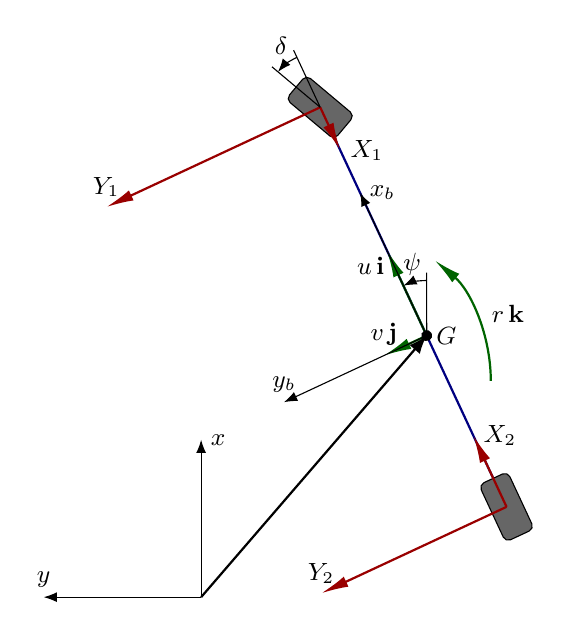
\begin{tikzpicture}[scale=2, x = {(0,1cm)}, y = {(-1cm,0)},
	force/.style={->, thick, red!60!black, >={Latex[length=10pt, width=4pt]}},
	vec/.style={->, thick, mgreen, >={Latex[length=10pt, width=4pt]}},
	aux/.style={thin},
	frame/.style={->,thin,>={Latex}},
	every node/.style={font=\small, text=black}
	]
	\definecolor{mgreen}{RGB}{0,100,0}
	\begin{scope}[rotate = 25,shift = {(-.3,-2)}]
		% Coordinates
		\coordinate (rear) at (0,0);
		\coordinate (G) at (1.2,0);
		\coordinate (front) at (2.8,0);
		
		% Main body line
		\draw[blue!50!black, thick] (rear) -- (front);
		
		% Rear wheel
		\draw[fill=black!60!white, draw=black, rounded corners=2pt]
		($(rear)+(-.2,.1)$) rectangle ($(rear)+(+.2,-.1)$);
		
		% Front wheel (rotated around its center)
		\begin{scope}[shift={(front)}, rotate=25]
			\draw[fill=black!60!white, draw=black, rounded corners=2pt]
			(-0.2,.1) rectangle (0.2,-.1);
		\end{scope}
		
		% Local axes at rear
		\draw[force] (rear) -- ++(.5,0) node[above,right] {$X_2$};
		\draw[force] (rear) -- ++(0,1.3) node[above] {$Y_2$};
		
		% Local axes at front
		\draw[force] (front) -- ++(-.3,0) node[right] {$X_1$};
		\draw[force] (front) -- ++(0,1.5) node[above] {$Y_1$};
		
		% Velocity vectors at G
		\draw[vec] (G) -- ++(.6,0) node[left, shift={(-.2,-.1)}] {$u\,\mathbf{i}$};
		\draw[vec] (G) -- ++(0,.3) node[above] {$v\,\mathbf{j}$};
		
		% Angular velocity
		\begin{scope}[rotate = -115]
			\draw[vec] 
			(-.1,.8) arc[start angle=0, end angle=50, radius=1]
			node[midway, right=2pt] {$r\,\mathbf{k}$};
		\end{scope}
		
		% G point
		\fill (G) circle (1pt) node[right] {$G$};
		
		% Body frame
		\draw[frame] (G) --++ (1,0) node[right] {$x_b$};
		\draw[frame] (G) --++ (0,1) node[above] {$y_b$};
		
		% Distances
		%			\draw[<->,>={Latex}] (3,-1) -- node[left] {$a_1$} (1.5,-1);
		%			\draw[<->,>={Latex}] (1.5,-1) -- node[left] {$a_2$} (0,-1);
		
		% Steering angle (auxiliary vertical line)
		\draw[aux] (front) -- ++(.4,0);
		\draw[aux] (front) -- ++({0.4*cos(25)}, {0.4*sin(25)});
		
		% Steering angle arc
		\draw[->,thin,>={Latex}] ([shift={(0.35,0)}]front) arc[start angle=0, end angle=25, radius=0.35];
		\node[left,shift={(.15,0)}] at ([shift={(0.35,0)}]front) {$\delta$};
		
		% Psi angle aux
		\draw[aux] (G) -- ++({0.4*cos(25)}, {-0.4*sin(25)});
		
		% Psi angle
		\draw[->,thin,>={Latex}] ([shift={({0.35*cos(25)},{-.35*sin(25)})}]G) arc[start angle=-25, end angle=0, radius=0.35];
		\node[left,shift={(.2,-.05)}] at ([shift={({0.35*cos(25)},{-.35*sin(25)})}]G) {$\psi$};
		
	\end{scope}
	\coordinate (ground) at (0,0);
	\draw[frame] (ground) --++ (1,0) node[right] {$x$};
	\draw[frame] (ground) --++ (0,1) node[above] {$y$};
	\draw[->,thick,>=Latex] (ground) --++ (G);
	%		\draw[->,thick,>=Latex] (ground) --++ (G) node[midway, shift={(0,-.3)}] {$\boldsymbol{p}$};
	
\end{tikzpicture}
	%\caption{Single Track model. The ground force acting on each axle is decomposed into longitudinal and lateral components, indicated by red arrows. The longitudinal components are part of the input vector $\bu$, encompassing both acceleration and braking forces, while the lateral components are computed using Pacejka's Magic Formula based on the vertical load and slip angle at each axle. The figure also depicts the fixed reference frame and the body reference frame, with the origin located at the vehicle's center of mass (CoM). The state variables $u$ and $v$ represent the longitudinal and lateral velocities of the CoM w.r.t. the body frame, while $r$ denotes the yaw rate. The angle $\psi$ is used to describe the orientation of the body frame w.r.t. the fixed frame.}
	\caption{Single Track model.}
	\label{fig:vehicle_model}
\end{figure}

\subsection{Stochastic vehicle dynamics}
\label{sec:stochastic_vehicle_dynamics}

We model the \emph{perturbed vehicle dynamics} as the following nonlinear continuous-time random dynamical system
\begin{align}
\dbx(t) = f(\bx(t), \bu(t)) + \bw(t),
\end{align}
where $\bu(t)$ are the deterministic control inputs, $\bw(t)$ is additive Gaussian white noise with zero mean and known covariance $\bQ(t)$, i.e. $\bw(t) \sim \calN(\bzero, \bQ(t))$, and $\bx(t)$ is the state vector.
Assuming a \emph{first-order} approximation for the disturbance propagation rule, $\bx(t)$ results in a Gaussian distribution with mean $\bmu(t)$ and covariance $\bP(t)$, so that $\bx(t)~\sim~\calN(\bmu(t), \bP(t))$.

Due to the symmetry of the probability density function (pdf) with respect to $\bmu(t)$, it is possible to represent the time evolution of the pdf as: i) the deterministic evolution of the mean $\bmu(t)$
\begin{align}\label{eq:meandynamics}
\dbmu(t) = f(\bmu(t), \bu(t)),
\end{align}
and ii) the time evolution of the state covariance matrix $\bP(t)$ along $\bmu(t)$, which can be expressed by the \emph{Lyapunov matrix differential equation}
\begin{align}\label{eq:dP}
\dbP(t) = \bA(t) \bP(t) + \bP(t) \bA^T(t) + \bQ(t),\quad \bP(0) = \bP_0 = \bP_0^T.
\end{align}
In~\eqref{eq:dP}, $\bP_0$ is the \emph{initial} state covariance and $\bA(t)$ is the usual shorthand notation for the Jacobian along the mean trajectory $\bmu(t)$, that is $\bA(t)=\frac{\pd f(\bmu, \bu)}{\pd \bmu}$.
%\bJ(\bmu(t),\bu(t))$, where $\bJ(\bx, \bu) = \frac{\pd f(\bx, \bu)}{\pd \bx}$.

As can be readily verified by differentiation~\cite{Gajic:LyapunovMatrixEquation:2010}, the analytical solution of~\eqref{eq:dP} has the form
\begin{align}\label{eq:P_STM}
\bP(t) = \bPhi(t,t_0) \bP_0 \bPhi^T(t,t_0)+\int_{t_0}^{t} \bPhi(t,\tau) \bQ(\tau) \bPhi^T(t,\tau) \dd \tau \quad \bP(0)=\bP_0,
\end{align}
where $\bPhi(t,t_0)$ is the \emph{state transition matrix}. This matrix encodes the evolution from $t_0$ to $t$ of a perturbation w.r.t. to the mean trajectory $\bmu(t)$. In symbols, $\barbx(t) = \bPhi(t,t_0) \barbx(t_0)$, with $\barbx(\cdot) =\bx(\cdot) - \bmu(\cdot) $. In turn, the evolution of $\bPhi(t,t_k)$ from a generic $t_k$ to $t$ is driven by the following differential equation
\begin{align}\label{eq:STM}
\dbPhi(t,t_k) = \bA(t)\bPhi(t,t_k), \quad \bPhi(t_k, t_k) = \bI.
\end{align}
In geometric and orbital mechanics, see e.g.~\cite{Maruskin:DynamicalSystemsGeometric:2018} or~\cite{Tapley:StatisticalOrbitDetermination:2004}, the usual choice for statistical trajectory determination is to employ~\eqref{eq:meandynamics} along with~\eqref{eq:P_STM} and~\eqref{eq:STM}. In our case, since we use collocation integrators for stochastic trajectory planning, we follow a more direct approach -- motivated by~\cite{Gillis:PracticalMethodsApproximate:2015} -- by directly employing~\eqref{eq:meandynamics} and~\eqref{eq:dP}.

Accordingly, the continuous-time stochastic trajectory planning can be framed as the following nonlinear optimal control problem
\begin{subequations}\label{eq:OCP}
\begin{align}
	\underset{\bmu(t), \bu(t), \bP(t)}{\text{minimize}} \quad & J(\bmu(t), \bu(t), \bP(t)) \label{eq:OCPcost} \\
	\text{s.t.} \quad \dbmu(t)           &= f(\bmu(t), \bu(t)) \label{eq:OCPdyn} \\
	\phantom{\text{s.t.} \quad} \bmu(0)  &= \bmu_0 \label{eq:OCPdynIC} \\
	\phantom{\text{s.t.} \quad} \dbP(t) &= \bA(t) \bP(t) + \bP(t) \bA^T(t) + \bQ(t) \label{eq:OCPdP} \\
	\phantom{\text{s.t.} \quad} \bP(0)  &= \bP_0 \succeq 0 \label{eq:OCPdPIC} \\ %& \phantom{\text{s.t.} \qquad} 0       \geq h_i(\bmu(t), \bu(t))
	%+ \overbrace{\gamma \bigg[\underbrace{\na^T_{\bx} h_i \bP(t) \na_{\bx} h_i}_{\text{variance of $h_i(\bx)$}}\bigg]^{\frac{1}{2}}}^{\text{safety margin}},
	\phantom{\text{s.t.} \qquad} 0&       \geq h_i(\bmu(t), \bu(t))
	+ \be_i(\bmu(t), \bu(t), \bP(t)),
	\quad i \in \calI \label{eq:OCPconstraints}
\end{align}
\end{subequations}
The cost function $J$ in~\eqref{eq:OCPcost} depends on the mean $\bmu(t)$, the controls $\bu(t)$ and the state covariance $\bP(t)$. The mean dynamics is expressed by~\eqref{eq:OCPdyn} with~\eqref{eq:OCPdynIC}, and the covariance dynamics is expressed by~\eqref{eq:OCPdP} with~\eqref{eq:OCPdPIC}. In eq.~\eqref{eq:OCPconstraints} the \emph{back-off terms} $\be_i$ account for the disturbances and serve the purpose of obtaining deterministic safety margins directly on $\bmu(t)$. $\calI$ is the set of indices defining the inequality constraints. The back-off terms stem from a linearization around the mean of the original \emph{chance constraint} on $\bx(t)$ expressed by $\Prob \{h_i(\bx) \leq 0\}\geq p$, where $p$ is the confidence level of constraint satisfaction. Explicitly, the back-off terms are given by
$\be_i = \gamma \sig_i$. The coefficient $\gamma = \Phi^{-1}(p)$ is the quantile function, where $\Phi(z)=\Prob \{Z\leq z\}$ is the cumulative distribution function (cdf) of a standard normal distribution $Z \sim \calN(0,1)$, and acts as a \emph{tuning knob}: the greater the confidence level $p$ required, the higher the gain $\ga$\footnote{For example, with $p=0.84$ $\ga = 1.0$, with $p=0.97$ $\ga = 2.0$, with $p=0.99$ $\ga = 3.0$}. The term $\sig_i = \big[\na^T_{\bx} h_i(\bmu) \bP(t) \na_{\bx} h_i(\bmu)\big]^{\frac{1}{2}}$ represents the standard deviation of the constraint $h_i(\bx)$ linearized around the mean, i.e. of random variable $h_i(\bmu)+\na^T_{\bx} h_i(\bmu) (\bx - \bmu)$, and follows immediately from the propagation rule of covariance.

\subsection{Discretization via direct collocation}
\label{sec:discretization}
The nonlinear optimal control problem~\eqref{eq:OCP} can be discretized by applying a suitable collocation integrator obtaining the following nonlinear program (NLP)
\begin{subequations}\label{eq:DOCP}
\begin{alignat}{3}
\underset{\bmu_k,\bxi_k, \bu_k, \bP_k,\bz_k}{\text{minimize}} \,
& & & J_k(\bmu_k,\bxi_k, \bu_k) & & \label{eq:DOCPcost} \\
\hspace*{-2.0 cm}\text{s.t.} \quad
& \bzero      & = & \; \bPsimu_k(\bmu_{k-1},\bmu_k,\bxi_k, \bu_k,\bz_k),
& \quad & k = 1,\ldots, N \label{eq:DOCPdyn} \\
& \bmu_0      & = & \; \bar{\bmu}_0
& & \label{eq:DOCPdynIC} \\
& \bzero      & = & \; \bPsiP_k(\bmu_k,\bxi_k, \bu_k, \bP_{k-1},\bP_k,\bSi_k,\bz_k),
& \quad & k = 1,\ldots, N \label{eq:DOCPdP} \\
& \bP_0       & = & \; \bar{\bP}_0 \succeq 0
& & \label{eq:DOCPdPIC} \\
& \bzero      & = & \; \bOm_k(\bmu_k,\bxi_k, \bu_k,\bz_k),
& \quad & k = 0,\ldots, N \label{eq:DOCPpath} \\
& 0           & \geq & \; h_i(\bmu_k, \bu_k, \bz_k) + \be_i(\bmu_k, \bu_k, \bP_k, \bz_k),
& \quad & k = 1,\ldots, N;\; i \in \calI \label{eq:DOCPconstraints}
\end{alignat}
\end{subequations}
To perform the discretization, the track centerline is parameterized using a curvilinear parameter $\alpha \in [0,1]$, and uniformly sampled at $N+1$ points $\alpha_0, \ldots, \alpha_N$.
Accordingly, $\bmu_k$ denotes the mean state at grid node $\alpha_k$, while the controls $\bu_k$ and the algebraic variables $\bz_k$ are assumed to be piecewise constant over each interval $[\al_k, \al_{k+1}]$.
The $\bz_k$'s are introduced as direct handles for physically meaningful quantities such contact forces. Similarly, $\bP_k$ represents the covariance matrix at the $k$-th node.
Following the direct collocation approach, both the mean and covariance state trajectories are approximated, in the $k$-th interval, with polynomials $\pi_k(\tau)$, defined on the unit interval $\tau\in[0,1]$, and then scaled to match the width $\nu_k$ of the corresponding time step. On the unit interval, we select $d$ collocation points $\tau_1, \ldots, \tau_d$, associated with as many collocation states. Accordingly, we define $\bxi_k$ and $\bSi_k$ as the mean states and covariance matrices at the $d$ collocation points within each interval $[\al_k, \al_{k+1}]$, respectively. Therefore, $\bxi_k =
(\bxi_{k,1}, \ldots, \bxi_{k,d})$, and similarly $\bSi_k=(\bSi_{k,1}, \ldots, \bSi_{k,d})$. Equations~\eqref{eq:DOCPdyn} and~\eqref{eq:DOCPdP} represent the collocation and continuity equations for mean and covariance, respectively, with initial conditions represented by~\eqref{eq:DOCPdynIC} and~\eqref{eq:DOCPdPIC}. Eqs.~\eqref{eq:DOCPpath} are path equality constraints and~\eqref{eq:DOCPconstraints} are the robustified inequality constraints.

In certain cases~\cite{Gillis:PracticalMethodsApproximate:2015}, positive-definiteness-preserving Lyapunov discretization schemes are used in~\eqref{eq:DOCPdP}. However, for sufficiently fine discretization, we found that integrating only the lower triangular part of $\bP(t)$ in~\eqref{eq:OCPdPIC}  (and reconstructing its strictly upper part accordingly), ensures that $\bP_k$ remain symmetric and positive definite when the initial $\bP_0$ is symmetric and positive definite. In all our tests direct collocation with cubic polynomial state representations and Gauss-Legendre collocation points provided accurate results.

\subsection{Robust friction limit constraint formulation}
\label{sec:FLC}
The model employs a tire formulation that neglects combined slip effects, i.e., it does not account for the simultaneous utilization of longitudinal and lateral tire forces. As a result, the optimal control problem must include an additional constraint to ensure that the total ground reaction forces remain within the bounds of the tire's adherence ellipse.

The base version of the constraint for each axle can be expressed as the following inequality depending on $\bx$ and $\bu$
\begin{equation}
	h^\textrm{FLC}_j(\bx,\bu) =  S_j(\bx,\bu) - 1 \leq 0, \qquad{(j=1,2)}
\label{eq:adherence_with_axle_saturation}
\end{equation}
where we introduced the \emph{axle saturation ratio} $S_j(\bx,\bu)$ as follows
\begin{equation}
	S_j(\bx,\bu) = \frac{ \left( \frac{X_j(\bx,\bu)}{\mu_{x,j}} \right)^2+ \left( \frac{Y_j(\bx,\bu)}{\mu_{y,j}}\right)^2}{Z_j^2(\bx,\bu)}.
\label{eq:axle_saturation}
\end{equation}
In~\eqref{eq:adherence_with_axle_saturation}, the superscript FLC denotes friction limit constraint, and $j=1,2$ refer the front and rear axle, respectively. In~\eqref{eq:axle_saturation}, $X_j$ and $Y_j$ denote the longitudinal and lateral components of the in-plane ground forces, respectively, as illustrated in Fig.~\ref{fig:vehicle_model}, while $Z_j$ represents the total vertical load acting on the axle.

From~\eqref{eq:axle_saturation} it is evident that $S_j(\bx,\bu)\in [0,1]$ indicates how close each configuration operates to the friction limit: $S_j=0$ when the overall grip demand is zero, while $S_j = 1$ when the point $\left(X_j, Y_j\right)$ lies exactly on the friction ellipse, i.e., under full saturation.
The points $\left(X_j,Y_j\right)$ are constrained to lie within an ellipse whose semi-axes are given by $\mu_{x,j}Z_j$ and $\mu_{y,j}Z_j$. The constraint, without the back-off term, is represented in the left panel of Fig.~\ref{fig:robust_constraints} by the solid line ellipse in the $X_jY_j$-plane.

To better clarify the effect of the back-off term on the constraint let us consider a combination of $\bx$, $\bu$, $P$ and $\ga^\textrm{FLC}_j$ so that $\be^\textrm{FLC}_j=0.2$. This implies that the semi-axes of the ellipse are reduced by a factor $\sqrt{1-\be^\textrm{FLC}_j} = \sqrt{0.8}$, as shown in the left panel of Fig.~\ref{fig:robust_constraints}, where the ellipse in dashed line delimits the available region with the back-off applied. This allows the optimizer to determine the most appropriate trade-off between the longitudinal force $X_j$ and the lateral force $Y_j$ --- often by reducing both components to some extent --- based on the specific requirements of the manoeuvre.

%The gradient of the constraint w.r.t. the state vector $\bx$, denoted by $\na_{\bx}h^\textrm{A}_j(\bmu)$, is used to evaluate the standard deviation $\sigma^\textrm{A}_j$ associated with the constraint. This gradient can be computed using the chain rule, as follows:
%\begin{equation}
%	\na_{\bx}h^\textrm{A}_j(\bmu,\bu) =
%	\frac{\pd h^\textrm{A}_j}{\pd X_j}\at_{\bmu,\bu}\na_{\bx}X_j(\bmu,\bu) +
%	\frac{\pd h^\textrm{A}_j}{\pd Y_j}\at_{\bmu,\bu}\na_{\bx}Y_j(\bmu,\bu) +
%	\frac{\pd h^\textrm{A}_j}{\pd Z_j}\at_{\bmu,\bu}\na_{\bx}Z_j(\bmu,\bu)
%\end{equation}
%where the first element is zero because $X_j$ is a function of the input vector $\bu$ only.

\begin{figure}
	\centering
	\adjustbox{valign=c}{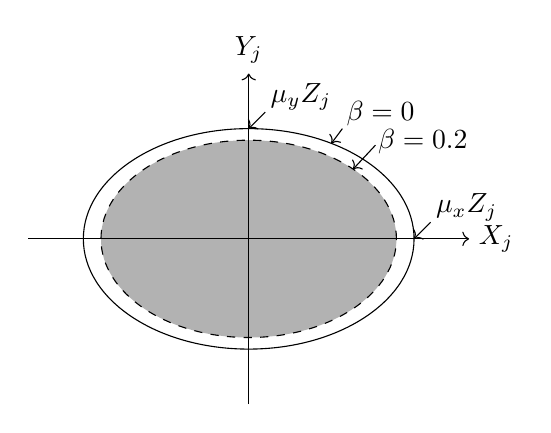
\begin{tikzpicture}[scale = .7]
	% Parameters
	\def\outerX{3}   % x radius of outer ellipse
	\def\outerY{2}   % y radius of outer ellipse
	\def\gap{0.2}    % distance between outer and inner ellipse
	\def\innerX{2.68}
	\def\innerY{1.79}
	
	% Draw outer ellipse
	\draw[] (0,0) ellipse [x radius=\outerX, y radius=\outerY];
	
	% Draw inner ellipse filled with color
	\fill[black!30] (0,0) ellipse [
	x radius={\innerX},
	y radius={\innerY}
	];
	\draw[dashed] (0,0) ellipse [
	x radius={\innerX},
	y radius={\innerY}
	];
	
	% Draw axes
	\draw[->] (-\outerX-1,0) -- (\outerX+1,0) node[right] {$X_j$};
	\draw[->] (0,-\outerY-1) -- (0,\outerY+1) node[above] {$Y_j$};
	
	% Arrows pointing to the ellipses
	\draw[->,thin] (1.7,2) -- ({\outerX*cos(60)},{\outerY*sin(60)}) node[midway, above right] {$\beta=0$};
	\draw[->,thin] (2.3,1.7) -- ({(\innerX)*cos(45)},{(\innerY)*sin(45)}) node[midway, right, shift={(0.05,.2)}] {$\beta=\gap$};
	
	% Arrows pointing to the ellipses
	\draw[->,thin] ({\outerX+.3},.3) -- (\outerX,0) node[midway, above right,shift={(.05,0)}] {$\mu_x Z_j$};
	\draw[->,thin] (.3,{\outerY+.3}) -- (0,\outerY) node[midway, above right,shift={(.05,0)}] {$\mu_y Z_j$};
	
\end{tikzpicture}}
	\hfill
	\adjustbox{valign=c}{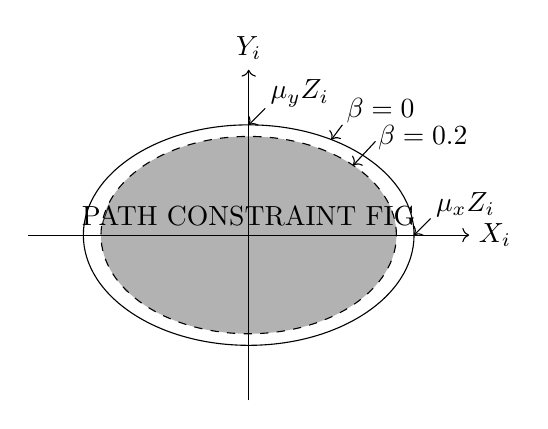
\begin{tikzpicture}[scale = .7]
	% Parameters
	\def\outerX{3}   % x radius of outer ellipse
	\def\outerY{2}   % y radius of outer ellipse
	\def\gap{0.2}    % distance between outer and inner ellipse
	\def\innerX{2.68}
	\def\innerY{1.79}
	
	% Draw outer ellipse
	\draw[] (0,0) ellipse [x radius=\outerX, y radius=\outerY];
	
	% Draw inner ellipse filled with color
	\fill[black!30] (0,0) ellipse [
	x radius={\innerX},
	y radius={\innerY}
	];
	\node[above] at (0,0) {PATH CONSTRAINT FIG};
	\draw[dashed] (0,0) ellipse [
	x radius={\innerX},
	y radius={\innerY}
	];
	
	% Draw axes
	\draw[->] (-\outerX-1,0) -- (\outerX+1,0) node[right] {$X_i$};
	\draw[->] (0,-\outerY-1) -- (0,\outerY+1) node[above] {$Y_i$};
	
	% Arrows pointing to the ellipses
	\draw[->,thin] (1.7,2) -- ({\outerX*cos(60)},{\outerY*sin(60)}) node[midway, above right] {$\beta=0$};
	\draw[->,thin] (2.3,1.7) -- ({(\innerX)*cos(45)},{(\innerY)*sin(45)}) node[midway, right, shift={(0.05,.2)}] {$\beta=\gap$};
	
	% Arrows pointing to the ellipses
	\draw[->,thin] ({\outerX+.3},.3) -- (\outerX,0) node[midway, above right,shift={(.05,0)}] {$\mu_x Z_i$};
	\draw[->,thin] (.3,{\outerY+.3}) -- (0,\outerY) node[midway, above right,shift={(.05,0)}] {$\mu_y Z_i$};
	
\end{tikzpicture}}
	\caption{Graphical representation of the two constraints analyzed in this section: the friction limit constraint in the $X_jY_j$ plane (left panel), and the track limit constraint in the $xy$ plane (right panel). In both figures, the filled gray area bounded by a dashed line indicates the accessible region in the presence of a back-off term.
	}
		%Graphical representation of the two constraints analyzed in the section. The left panel shows the friction limit constraint in the plane $X_j-Y_j$. The ellipse in solid line, whose semi-axes are given by $\mu_{x,j}Z_j$ and $\mu_{y,j}Z_j$, represents the border of the available region for the base constraint, without back-off. The ellipse in dashed line delimits the available region when a back-off $\be^\textrm{FLC}_j=0.2$ is present. This ellipse has its semi-axes reduced by a factor $\sqrt{1-\be^\textrm{FLC}_j}$ w.r.t. the one in solid line.}
	\label{fig:robust_constraints}
\end{figure}

\subsection{Robust track limit constraint formulation}
\label{sec:TLC}
A track limit constraint is required to ensure that the vehicle remains within the circuit boundaries. The formulation adopted introduces an algebraic variable $e$, which satisfies the following constraint:
\begin{equation}
	\begin{Bmatrix}
		x\\y
	\end{Bmatrix}
	-\boldsymbol{c} - e\bn=\boldsymbol{0} \label{eq:onplane_constraint}
\end{equation}
%\begin{equation}
%	\bp-\boldsymbol{c}_k - e_k\bn_k=\boldsymbol{0} \label{eq:onplane_constraint}
%\end{equation}
where $\boldsymbol{c}$ indicates the position of the centerline, and $\bn$ is the unit normal vector to the centerline. Equation~\eqref{eq:onplane_constraint} constraints the CoM of the vehicle to lie on the vertical plane defined by the unit normal vector $\bn$. The previously introduced algebraic variable $e$ is further constrained to take values between $e_\textrm{min}$ and $e_\textrm{max}$, which are determined based on the width of the circuit and the vehicle's front and rear tracks.

In order to take into account the back-off terms, the maximum and minimum values are modified coherently, so that:
\begin{equation}
	e_\textrm{min} + \be^\textrm{TLC} \leq e \leq e_\textrm{max} - \be^\textrm{TLC}\label{eq:TLC}
\end{equation}
where $\be^\textrm{TLC}$ is computed by considering that the gradient of the constraint w.r.t. the state vector $\na_{\bx}h^\textrm{TLC}$ depends solely on $\bn$.
%Adding a back-off to this constraint produces the same effect as an increase of the front and rear tracks of the vehicle does. 
\section{Open-loop planning via H-steps ahead predictions}
\label{sec:open_loop_planning}
In this section, we address the problem of planning under uncertainty for a stochastic system. 
At each grid point $k$ of the discretized trajectory the covariance matrix is propagated in a feed-forward fashion for a fixed prediction horizon of $H$ steps.
In the planning problem, we conservatively evaluate the maximum propagation of the covariance, that is, the matrix evolved over $H$ steps, to ensure the tightest possible enforcement of constraints. This maximizes the robustness of the resulting solution, as the constraint back-off is evaluated in the worst-case scenario within the prediction horizon.

To enable this, we associate multiple versions of the covariance matrix with each grid point. Specifically, $H+1$ instances of the matrix $\bP$ are maintained at each step. To this sake we introduce the notation $\bP_k^j$, where $j = 0, \ldots, H$, and $\bP_k^j$ represents the version of the covariance matrix at step $k$ that was initialized $j$ steps earlier. Hence, $\bP_k^0$ originates at node $k$ itself and will be propagated forward and employed in subsequent steps (exactly when evolved as $\bP_{k+H}^H$ ), while $\bP_k^H$ is the instance that originated $H$ steps earlier and is the most propagated one at step $k$. 

The repeated initialization of the covariance matrix at each step is necessary to prevent its unbounded growth, as we assume that the system evolves without feedback control.
In the absence of feedback, the uncertainty on the position and orientation of the body frame accumulates along the track, leading to a severe and unrealistic degradation of the covariance matrix conditioning.
For this reason, the propagation horizon in this open-loop setting is a critical design parameter.
We bound the number of steps $H$ to realistically capture the evolution of disturbances occurring prior to any corrective driver response.
 
This approach requires modifications to the formulation~\eqref{eq:DOCP} introduced in Section~\ref{sec:discretization}. In particular, Eqs.~\eqref{eq:DOCPdP}, \eqref{eq:DOCPdPIC}, and \eqref{eq:DOCPconstraints} are replaced by Eqs.~\eqref{eq:DOCPdPopenloop}, \eqref{eq:DOCPdPinitopenloop}, and \eqref{eq:DOCPconstraintsopenloop}. Equation~\eqref{eq:DOCPdPopenloop} collects the continuity and collocation equations for all versions of the covariance matrix propagated from previous steps. To support the evolution of $H$ versions, we introduce $H \times d$ matrices $\bSi_k^j = (\bSi_{k,1}^j, \ldots, \bSi_{k,d}^j)$, representing the collocation values of each version $j$ of the covariance matrix within interval $k$.


%The proposed approach requires the presence of $H+1$ versions of the matrix $\bP$ at each grid point of the discretized problem. One of these versions is initialized with $\bar{\bP}_0$, while the others represent the evolution of matrices that were initialized at previous grid points, from 1 to $H$ steps earlier. This ensures that at each step it is possible to find a covariance matrix evolved for $H$ steps and use it to robustify the constraints. The initialization of the covariance matrix is necessary due to its divergent dynamics. In fact, without a feedback control, the error on the position and orientation of the body reference frame can only increase along the track, compromising the conditioning of the matrix.
%
%Introducing the versioning of the covariance matrix approach requires a modification of the Equations described in Section~\ref{sec:discretization}. In particular Eqs.~\eqref{eq:DOCPdP}, \eqref{eq:DOCPdPIC}, and \eqref{eq:DOCPconstraints} are replaced by Eqs.~\eqref{eq:DOCPdPopenloop}, \eqref{eq:DOCPdPinitopenloop}, and \eqref{eq:DOCPconstraintsopenloop}. Eq.~\eqref{eq:DOCPdPopenloop} collects the continuity and collocation Equations for all the versions of the covariance matrix that have propagated from the previous step. To account for the evolution of $H$ matrices, it is necessary to introduce $H\times d$ matrices $\bSi_k^j=(\bSi_{k,1}^j, \ldots, \bSi_{k,d}^j)$, which represent the values of each matrix version at the collocation points.

The specific formulation is expressed as follows:
\begin{subequations}\label{eq:DOCPopenloop}
\begin{alignat}{3}
	\underset{\bmu_k,\bxi_k, \bu_k, \bP_k,\bz_k}{\text{minimize}} \,
	& & & J_k(\bmu_k,\bxi_k, \bu_k) & & \label{eq:DOCPcostopenloop} \\
	\hspace*{-2.0 cm}\text{s.t.} \quad
	& \bzero      & = & \; \bPsimu_k(\bmu_{k-1},\bmu_k,\bxi_k, \bu_k,\bz_k),
	& \quad & k = 1,\ldots, N \label{eq:DOCPdynopenloop} \\
	& \bmu_0      & = & \; \bar{\bmu}_0
	& & \label{eq:DOCPdynICopenloop} \\
	& \bzero      & = & \; \bPsiP_k(\bmu_k,\bxi_k, \bu_k, \bP_{k-1}^{j-1},\bP_k^j,\bSi_k^j,\bz_k),
	& \quad & \substack{k = 1,\ldots, N; \; \\ j=1,\ldots,H;\;} \label{eq:DOCPdPopenloop} \\
	& \bP_k^0       & = & \; \bar{\bP}_0 \succeq 0
	& \quad & k = 1,\ldots, N; \; \label{eq:DOCPdPinitopenloop} \\
	& \bzero      & = & \; \bOm_k(\bmu_k,\bxi_k, \bu_k,\bz_k),
	& \quad & k = 0,\ldots, N \label{eq:DOCPpathopenloop} \\
	& 0           & \geq & \; h_i(\bmu_k, \bu_k, \bz_k) + \be_i(\bmu_k, \bu_k, \bP_k^H, \bz_k),
	& \quad & k = 1,\ldots, N;\; i \in \calI \label{eq:DOCPconstraintsopenloop}
\end{alignat}
\end{subequations}
Equation~\eqref{eq:DOCPdPinitopenloop} defines the initialization of the appropriate covariance matrix version at step $k$, while Eq.~\eqref{eq:DOCPconstraintsopenloop} specifies that the back-off term in the constraints is computed using the most propagated version, $\bP^H_k$. A schematic illustration of the management of the $H+1$ covariance matrix instances is provided in Figure~\ref{fig:DOCPgrid}. The dashed rectangle highlights the $k$-th discretization step, where the constraints are evaluated. At each grid point, two particular versions of the covariance matrix are emphasized: $\bP^0_k$ (red node), representing the instance to be initialized at that step, and $\bP^H_k$ (green node), corresponding to the version that has been propagated over the full horizon of $H$ steps and is used to robustify the constraints in Eq.~\eqref{eq:DOCPconstraintsopenloop}.



%Eq.~\eqref{eq:DOCPdPinitopenloop} is used to initialize the correct version at the $k$-th step while Eq.~\eqref{eq:DOCPconstraintsopenloop} specify that the back-off term of the constraints is evaluated with the most propagated covariance matrix version, $\bP^H_k$.
%A schematic representation of the approach used to manage the $H+1$ versions of the covariance matrix is shown in Figure \ref{fig:DOCPgrid}, where the dashed rectangle represent the $k$-th step at which the constraints are being formulated. At each grid point, two versions of the covariance matrix are highlighted: $\bP^0_k$ (red node), which is the version to be initialized, and $\bP^H_k$ (green node), which is the most propagated version used to formulate the robust constraints in Eq.~\eqref{eq:DOCPconstraintsopenloop}.
\def\version{marco}
\ifdefstring{\version}{matteo}{
\begin{figure}
	\centering
	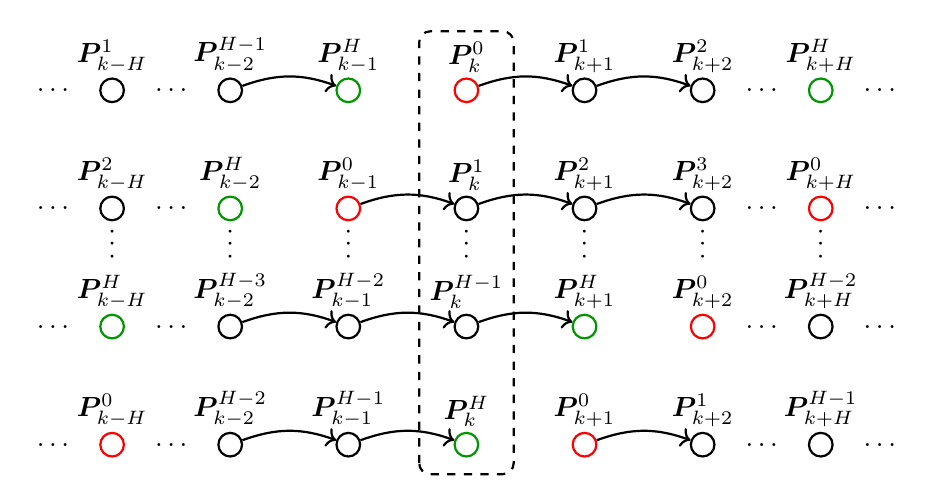
\begin{tikzpicture}[%
	smallnode/.style={%
		circle, draw, minimum size=3mm, inner sep=0pt
	},
	r_smallnode/.style={%
		circle, draw, minimum size=3mm, inner sep=0pt, red
	},
	g_smallnode/.style={%
		circle, draw, minimum size=3mm, inner sep=0pt, mygreen
	},
	every path/.style={->, thick},
	x=1.5cm, y=1.5cm
	]
	
	\newcommand{\Plab}[2]{\bP^{#2}_{#1}}
	\definecolor{mygreen}{RGB}{0 150 0}
	
	% Nodes
	% First row
	\node[smallnode, label={[label distance=-2pt]above:\(\Plab{k-2}{H-2}\)}] (Pk-2H-2) at (1,0) {};
	\node[smallnode, label={[label distance=-2pt]above:\(\Plab{k-1}{H-1}\)}] (Pk-1H-1) at (2,0) {};
	\node[g_smallnode, label={[label distance=-2pt]above:\(\Plab{k}{H}\)}] (PkH) at (3,0) {};
	\node[r_smallnode, label={[label distance=-2pt]above:\(\Plab{k+1}{0}\)}] (Pk+10) at (4,0) {};
	\node[smallnode, label={[label distance=-2pt]above:\(\Plab{k+2}{1}\)}] (Pk+21) at (5,0) {};
	
	\draw[bend left=20] (Pk-2H-2) to (Pk-1H-1);
	\draw[bend left=20] (Pk-1H-1) to (PkH);
	\draw[bend left=20] (Pk+10) to (Pk+21);
	
	\node[r_smallnode, label={[label distance=-2pt]above:\(\Plab{k-H}{0}\)}] (Pk-H0) at (0,0) {};
	\node[label={center:\(\dots\)}] (dots10) at (-.5, 0) {};
	\node[label={center:\(\dots\)}] (dots11) at (.5, 0) {};
	\node[smallnode, label={[label distance=-2pt]above:\(\Plab{k+H}{H-1}\)}] (Pk+HH-1) at (6,0) {};
	\node[label={center:\(\dots\)}] (dots12) at (5.5, 0) {};
	\node[label={center:\(\dots\)}] (dots13) at (6.5, 0) {};
	% Second row
	\node[smallnode, label={[label distance=-2pt]above:\(\Plab{k-2}{H-3}\)}] (Pk-2H-3) at (1,1) {};
	\node[smallnode, label={[label distance=-2pt]above:\(\Plab{k-1}{H-2}\)}] (Pk-1H-2) at (2,1) {};
	\node[smallnode, label={[label distance=-2pt]above:\(\Plab{k}{H-1}\)}] (PkH-1) at (3,1) {};
	\node[g_smallnode, label={[label distance=-2pt]above:\(\Plab{k+1}{H}\)}] (Pk+1H) at (4,1) {};
	\node[r_smallnode, label={[label distance=-2pt]above:\(\Plab{k+2}{0}\)}] (Pk+20) at (5,1) {};
	
	\draw[bend left=20] (Pk-2H-3) to (Pk-1H-2);
	\draw[bend left=20] (Pk-1H-2) to (PkH-1);
	\draw[bend left=20] (PkH-1) to (Pk+1H);
	
	\node[g_smallnode, label={[label distance=-2pt]above:\(\Plab{k-H}{H}\)}] (Pk-HH) at (0,1) {};
	\node[label={center:\(\dots\)}] (dots20) at (-.5, 1) {};
	\node[label={center:\(\dots\)}] (dots21) at (.5, 1) {};
	\node[smallnode, label={[label distance=-2pt]above:\(\Plab{k+H}{H-2}\)}] (Pk+HH-2) at (6,1) {};
	\node[label={center:\(\dots\)}] (dots22) at (5.5, 1) {};
	\node[label={center:\(\dots\)}] (dots23) at (6.5, 1) {};
	
	% dots row
	\node[label={center,rotate=90:\(\dots\)}] (dots1) at (0, 1.7) {};
	\node[label={center,rotate=90:\(\dots\)}] (dots2) at (1, 1.7) {};
	\node[label={center,rotate=90:\(\dots\)}] (dots3) at (2, 1.7) {};
	\node[label={center,rotate=90:\(\dots\)}] (dots4) at (3, 1.7) {};
	\node[label={center,rotate=90:\(\dots\)}] (dots5) at (4, 1.7) {};
	\node[label={center,rotate=90:\(\dots\)}] (dots6) at (5, 1.7) {};
	\node[label={center,rotate=90:\(\dots\)}] (dots7) at (6, 1.7) {};
	
	% Third row
	\node[g_smallnode, label={[label distance=-2pt]above:\(\Plab{k-2}{H}\)}] (Pk-2H) at (1,2) {};
	\node[r_smallnode, label={[label distance=-2pt]above:\(\Plab{k-1}{0}\)}] (Pk-10) at (2,2) {};
	\node[smallnode, label={[label distance=-2pt]above:\(\Plab{k}{1}\)}] (Pk1) at (3,2) {};
	\node[smallnode, label={[label distance=-2pt]above:\(\Plab{k+1}{2}\)}] (Pk+12) at (4,2) {};
	\node[smallnode, label={[label distance=-2pt]above:\(\Plab{k+2}{3}\)}] (Pk+23) at (5,2) {};
	
	\draw[bend left=20] (Pk-10) to (Pk1);
	\draw[bend left=20] (Pk1) to (Pk+12);
	\draw[bend left=20] (Pk+12) to (Pk+23);
	
	\node[smallnode, label={[label distance=-2pt]above:\(\Plab{k-H}{2}\)}] (Pk-H2) at (0,2) {};
	\node[label={center:\(\dots\)}] (dots30) at (-.5, 2) {};
	\node[label={center:\(\dots\)}] (dots31) at (.5, 2) {};
	\node[r_smallnode, label={[label distance=-2pt]above:\(\Plab{k+H}{0}\)}] (Pk+H0) at (6,2) {};
	\node[label={center:\(\dots\)}] (dots32) at (5.5, 2) {};
	\node[label={center:\(\dots\)}] (dots33) at (6.5, 2) {};
	
	% Fourth row
	\node[smallnode, label={[label distance=-2pt]above:\(\Plab{k-2}{H-1}\)}] (Pk-2H-1) at (1,3) {};
	\node[g_smallnode, label={[label distance=-2pt]above:\(\Plab{k-1}{H}\)}] (Pk-1H) at (2,3) {};
	\node[r_smallnode, label={[label distance=-2pt]above:\(\Plab{k}{0}\)}] (Pk0) at (3,3) {};
	\node[smallnode, label={[label distance=-2pt]above:\(\Plab{k+1}{1}\)}] (Pk+11) at (4,3) {};
	\node[smallnode, label={[label distance=-2pt]above:\(\Plab{k+2}{2}\)}] (Pk+22) at (5,3) {};
	
	\draw[bend left=20] (Pk-2H-1) to (Pk-1H);
	\draw[bend left=20] (Pk0) to (Pk+11);
	\draw[bend left=20] (Pk+11) to (Pk+22);
	
	\node[smallnode, label={[label distance=-2pt]above:\(\Plab{k-H}{1}\)}] (Pk-H1) at (0,3) {};
	\node[label={center:\(\dots\)}] (dots40) at (-.5, 3) {};
	\node[label={center:\(\dots\)}] (dots41) at (.5, 3) {};
	\node[g_smallnode, label={[label distance=-2pt]above:\(\Plab{k+H}{H}\)}] (Pk+HH) at (6,3) {};
	\node[label={center:\(\dots\)}] (dots42) at (5.5, 3) {};
	\node[label={center:\(\dots\)}] (dots43) at (6.5, 3) {};
	
	% Dashed rectangle
	\draw[dashed, thick, rounded corners] (2.6,-.25) rectangle (3.4,3.5);
	
\end{tikzpicture}
	\caption{Schematic representation of the continuity and initialization equations associated with the $H+1$ propagated instances of the covariance matrix introduced in problem~\eqref{eq:DOCPopenloop}. The dashed rectangle highlights the $k$-th discretization step, at which the robust constraints are enforced. Each node corresponds to a specific covariance matrix, where the subscript denotes the current grid index and the superscript indicates the number of propagation steps since initialization. At each step, two key instances are emphasized: the matrix to be initialized at that step (red node), and the matrix that has been propagated over $H$ steps (green node), which is used in the evaluation of the constraint backoff.}
	%\caption{Schematic representation of the continuity and initialization Equations for the $H+1$ versions of the covariance matrix introduced in the discretized OCP. The dashed rectangle indicate the $k$-th step, in which the constraints are formulated. Each node represents a covariance matrix, labeled such that the subscript denotes the current grid step, while the superscript indicates the number of propagation steps it has undergone. At each step, two nodes are highlighted: the covariance matrix to be initialized (red node) and the matrix that has been propagated for $H$ steps (green node), which is used to formulate the robust constraints.}
	\label{fig:DOCPgrid}
\end{figure}
}{}

\ifdefstring{\version}{marco}{
\begin{figure}
	\centering
	\definecolor{mygreen}{RGB}{0,150,0}
	\begin{tikzpicture}[
	smallnode/.style={circle, draw, minimum size=3mm, inner sep=0pt},
	r_smallnode/.style={circle, draw=red, minimum size=3mm, inner sep=0pt},
	g_smallnode/.style={circle, draw=mygreen, minimum size=3mm, inner sep=0pt},
	r_hatnode/.style={
		circle, draw=red, pattern=north east lines, pattern color=red,
		minimum size=3mm, inner sep=0pt},
	g_hatnode/.style={
		circle, draw=mygreen, pattern=north east lines, pattern color=mygreen,
		minimum size=3mm, inner sep=0pt},
	every path/.style={->, thick},
	x=1.4cm, y=1.2cm
	]
	
	% ROW j = 0 (y=3)
	\node[r_hatnode, label={[label distance=-2pt]above:\(\bP_{k-3}^0\)}] (P00) at (1,3) {};
	\node[smallnode, label={[label distance=-2pt]above:\(\bP_{k-2}^1\)}] (P11) at (2,3) {};
	\node[smallnode, label={[label distance=-2pt]above:\(\bP_{k-1}^2\)}] (P22) at (3,3) {};
	\node[g_hatnode, label={[label distance=-2pt]above:\(\bP_k^3\)}] (P33) at (4,3) {};
	\node[r_hatnode, label={[label distance=-2pt]above:\(\bP_{k+1}^0\)}] (P44) at (5,3) {};
	\node[smallnode, label={[label distance=-2pt]above:\(\bP_{k+2}^1\)}] (P55) at (6,3) {};
	
	% ROW j = 1 (y=2)
	\node[r_hatnode, label={[label distance=-2pt]above:\(\bP_{k-2}^0\)}] (P10) at (2,2) {};
	\node[smallnode, label={[label distance=-2pt]above:\(\bP_{k-1}^1\)}] (P21) at (3,2) {};
	\node[smallnode, label={[label distance=-2pt]above:\(\bP_k^2\)}] (P32) at (4,2) {};
	\node[g_hatnode, label={[label distance=-2pt]above:\(\bP_{k+1}^3\)}] (P43) at (5,2) {};
	\node[r_hatnode, label={[label distance=-2pt]above:\(\bP_{k+2}^0\)}] (P54) at (6,2) {};
	\node[smallnode, label={[label distance=-2pt]above:\(\bP_{k+3}^1\)}] (P65) at (7,2) {};
	
	
	% ROW j = 2 (y=1)
	\node[r_hatnode, label={[label distance=-2pt]above:\(\bP_{k-1}^0\)}] (P20) at (3,1) {};
	\node[smallnode, label={[label distance=-2pt]above:\(\bP_k^1\)}] (P31) at (4,1) {};
	\node[smallnode, label={[label distance=-2pt]above:\(\bP_{k+1}^2\)}] (P42) at (5,1) {};
	\node[g_hatnode, label={[label distance=-2pt]above:\(\bP_{k+2}^3\)}] (P53) at (6,1) {};
	\node[r_hatnode, label={[label distance=-2pt]above:\(\bP_{k+3}^0\)}] (P64) at (7,1) {};
	\node[smallnode, label={[label distance=-2pt]above:\(\bP_{k+4}^1\)}] (P75) at (8,1) {};
	
	% ROW j = 3 (y=0)
	\node[r_hatnode, label={[label distance=-2pt]above:\(\bP_k^0\)}] (P30) at (4,0) {};
	\node[smallnode, label={[label distance=-2pt]above:\(\bP_{k+1}^1\)}] (P41) at (5,0) {};
	\node[smallnode, label={[label distance=-2pt]above:\(\bP_{k+2}^2\)}] (P52) at (6,0) {};
	\node[g_hatnode, label={[label distance=-2pt]above:\(\bP_{k+3}^3\)}] (P63) at (7,0) {};
	\node[r_hatnode, label={[label distance=-2pt]above:\(\bP_{k+4}^0\)}] (P74) at (8,0) {};
	\node[smallnode, label={[label distance=-2pt]above:\(\bP_{k+5}^1\)}] (P85) at (9,0) {};
	
	
	% ARROWS
	\draw (P00) -- (P11);
	\draw (P11) -- (P22);
	\draw (P22) -- (P33);
	\draw (P22) -- (P33);
	
	\draw (P44) -- (P55);
	\draw[dashed,->] (P55) -- ++(1,0);
	
	\draw (P10) -- (P21);
	\draw (P21) -- (P32);
	\draw (P32) -- (P43);
	\draw (P54) -- (P65);
	\draw[dashed,->] (P65) -- ++(1,0);
	
	
	\draw (P20) -- (P31);
	\draw (P31) -- (P42);
	\draw (P42) -- (P53);
	\draw (P64) -- (P75);
	\draw[dashed,->] (P75) -- ++(1,0);
	
	\draw (P30) -- (P41);
	\draw (P41) -- (P52);
	\draw (P52) -- (P63);
	
	\draw (P74) -- (P85);
	\draw[dashed,->] (P85) -- ++(1,0);
	
	% Dashed box around column k (x=4)
	\draw[dashed, thick, rounded corners] (3.6,-0.5) rectangle (4.4,3.7);
	
	% Top axis labels
	\node at (0, 4.3) {\scriptsize \(\cdots\)};
	\node at (1, 4.3) {\scriptsize \(k-3\)};
	\node at (2, 4.3) {\scriptsize \(k-2\)};
	\node at (3, 4.3) {\scriptsize \(k-1\)};
	\node (knode) at (4, 4.3) {\scriptsize \(k\)};
	\node at (5, 4.3) {\scriptsize \(k+1\)};
	\node at (6, 4.3) {\scriptsize \(k+2\)};
	\node at (7, 4.3) {\scriptsize \(k+3\)};
	\node at (8, 4.3) {\scriptsize \(k+4\)};
	\node at (9, 4.3) {\scriptsize \(\cdots\)};
	
	% Wiggly arrow from label to top edge of dashed box
	\draw[->, thick, decorate, decoration={snake, amplitude=0.25mm, segment length=2.5mm}]
	(knode.south) -- (4, 3.8);
	
	% Legend box (top right)
	%\begin{scope}[shift={(6.5,2.5)}]
	%    \node[r_smallnode] (r) at (0,0) {};
	%    \node[anchor=west] at (0.4,0) {\scriptsize Initialized matrix \(\bP_k^0\)};
	%
	%    \node[g_smallnode] (g) at (0,-0.8) {};
	%    \node[anchor=west] at (0.4,-0.8) {\scriptsize Most propagated matrix \(\bP_k^3\)};
	%\end{scope}
	
\end{tikzpicture}
	\caption{Schematic representation (depicted for $H=3$) of the continuity and initialization equations associated with the $H+1$ propagated instances of the covariance matrix introduced in problem~\eqref{eq:DOCPopenloop}. The dashed rectangle highlights the $k$-th discretization step, at which the robust constraints are enforced. Each node corresponds to a specific covariance matrix, where the subscript denotes the current grid index and the superscript indicates the number of propagation steps since initialization. At each step, two key instances are emphasized: the matrix to be initialized at that step (red node), and the matrix that has been propagated over $H$ steps (green node), which is used in the evaluation of the constraint backoff.}
	%\caption{Schematic representation of the continuity and initialization Equations for the $H+1$ versions of the covariance matrix introduced in the discretized OCP. The dashed rectangle indicate the $k$-th step, in which the constraints are formulated. Each node represents a covariance matrix, labeled such that the subscript denotes the current grid step, while the superscript indicates the number of propagation steps it has undergone. At each step, two nodes are highlighted: the covariance matrix to be initialized (red node) and the matrix that has been propagated for $H$ steps (green node), which is used to formulate the robust constraints.}
	\label{fig:DOCPgrid}
\end{figure}
}{}

%for back-off calculations
\section{Closed-loop uncertainty-aware planning over the full horizon}
\label{sec:closed_loop_planning}

The second approach plans over the full horizon while incorporating a feedback policy that mimics the driver's closed-loop behavior. This enables a more realistic propagation of the uncertainty encoded in the covariance matrix $\bP$, preventing its uncontrolled growth through the stabilizing effect of the driver's feedback.

The approach is based on the three following steps: i) A nominal time-optimal trajectory is planned: this will be referred to as nominal feed-forward optimal trajectory. This is the trajectory a driver should follow in the ideal situation of a world without uncertainty. Therefore, in this step the mean trajectory is the actual trajectory a deterministic vehicle dynamics would trace. ii) A closed-loop controller mimicking the driver's action is computed which stabilizes the nominal feed-forward optimal trajectory computed at step i). We assume a discrete time-varying Linear Quadratic Regulator (LQR) controller is a good approximation of how an expert driver can track a prescribed trajectory. iii) In the last step the stochastic framework is reintroduced and the time-optimal planning problem is robustified using the Lyapunov framework. The main idea is to \emph{re-plan} a mean trajectory of a stochastic system such that, a time-varying LQR controller that aims at stabilizing it, is able to properly tame the propagation of the uncertainty. This amounts to ensuring that the robustified path constraints are satisfied. More specifically, this implies two key aspects: first, that the covariance matrix is propagated accounting explicitly for the controlled system dynamics; and second, that the path constraints are robustly satisfied by incorporating the covariance estimation propagated through the closed-loop controlled system. Some aspects that may initially appear technical are in fact essential. In this third step, not only are states and controls re-planned, but also the time-varying LQR gains. In fact, they need to explicitly account for the changed requirements associated with stabilizing a trajectory different from the nominal one, which must now satisfy the robustified constraints.
\subsection{Suspension Analysis}
\label{sec:suspanal}
The suspensions connect the chassis to the unsprung masses. This connection cannot be described by an elementary joint, such as prismatic or revolute. Therefore, a set of six variables $q_{bh}$, that parameterize a homogeneous transformation matrix, is necessary. The transformation can be realized by composing three translations and three rotations (the ZXY Euler sequence was selected) using the global Product of Exponentials (PoE) formula~\cite{Murray:book:1994}, which reads: \begin{equation}\label{eqn:PoE}
	g_{bh}=e^{\hat{Y}_1q_{bh,1}}\cdots e^{\hat{Y}_6q_{bh,6}} g_{bh}(0),
\end{equation}
where the offset $g_{bh(0)}=I$ and $Y_i=e_i$, with $e_i\in\bbR^6$ are the six normalized screw vectors (canonical basis elements in $\bbR^6$) associated with the Cartesian coordinates and the Euler ZXY angles in $q_{bh}$.
Clearly, the six components of $q_{bh}$ are not independent; the modeled suspension is, in fact, a double wishbone that has: 2 DoFs for wheels that can steer, and 1 DoF otherwise.
In this case, both axles have wheels that can steer; hence, a pair of independent variables ($z;\delta $) is associated with each wheel.
A detailed analysis is omitted here for the sake of brevity. The interested reader is referred to~\cite{Domenighini:Designs:2023} for a similar treatment using the PoE formalism.

%As mentioned in the previous sections, $z$ represents the variation of the distance between the two attachment points of the spring-damper system, positive when the distance increases and negative when it decreases, while $\delta$ represents the motion of the steering rod attachment point to the chassis along its local $y$ axis (frame $\sref{B}$). Considering that the type of the suspension is known, six scalar equations of constraints can be expressed implicitly as $F(q_{bh};z,\delta)=0\in \bbR^6$.
%
%To find an explicit relation between inputs $(z,\delta)$ and outputs $q_{bh}$, the constraint equations are solved on a grid of pairs $(z^{(p)},\delta^{(l)})$, where $p = 1,\dots,N$ and $l = 1,\dots,M$. Then, the data are fitted (in the least-squares sense) with a 2D regression polynomial $q_{bh}(z,\delta)$ as follows:
%\begin{equation}\label{eqn:poly}
%	q_{bh,i}(z,\delta)=\sum_{r=0}^{3} \sum_{s=0}^{3-r} a_{{rs},i} z^r \delta^s.
%\end{equation}
%For the purpose a polynomial of degree three is sufficiently accurate. Now is possible to express the homogeneous transformation $g_{bh}\bigl(q_{bh}(z,\delta)\bigr)$ and to compute the twist $V_{bh}$ and $\dot{V}_{bh}$ as functions of $(z,\delta)$ and their derivatives. We start from:
%\begin{equation}\label{eqn:Jbh}
%	V_{bh}=\sum_{i=1}^6J_{bh,i}\dot{q}_{bh,i},
%\end{equation}
%where $J_{bh}$ is the \emph{geometric Jacobian} of the suspension joint relative to $q_{bh}$. Then, following the procedure thoroughly described in~\cite[Sec. 2.2]{Domenighini:Designs:2023}, it is possible to obtain %
%assumed with independent components. Each column of $J_{bh}$ can be computed based on the PoE formula \eqref{eqn:PoE}. For the $i$-th column, we have $J_{bh,i}=A_i^{-1}Y_i$, with $A_6 = I_{6\times 6}$ and $A_i=\Ad_{e^{\hat{Y}_{i}q_{bh,i}}\cdots e^{\hat{Y}_6q_{bh,6}}}$, $i = 1, \dots, 5$. The \emph{Adjoint operator} $\Ad_g$ has been defined as the $6\times6$ matrix satisfying $Y=\Ad_gX$ whenever $\hat{Y}=g\hat{X}g^{-1}$, so that, if $g=\left[\begin{smallmatrix}R&d\\0^T&1\end{smallmatrix}\right]$, then $\Ad_g=\left[\begin{smallmatrix}R&\hat{d}R\\0&R\end{smallmatrix}\right]$.\\
%As a function of $(z,\delta)$, $\dot{q}_{bh,i}$ can be expressed as follows:
%\begin{equation}\label{eqn:dt_qbh}
%	\dot{q}_{bh,i}=\frac{\partial}{\partial z}q_{bh,i}\dot{z}+\frac{\partial}{\partial\delta}q_{bh,i}\dot{\delta},
%\end{equation}
%where the (geometric) partial derivatives $\frac{\partial}{\partial z}q_{bh,i}$ and $\frac{\partial}{\partial\delta}q_{bh,i}$ are obtained by differentiating Eq.~\eqref{eqn:poly}.
%Then, by defining the Jacobians with respect to the true independent variables $z$ and $\delta$ as follows
%\begin{align}\label{eqn:Jbh,z}
%	J_{bh,z}=\sum_{i=1}^6J_{bh,i}\frac{\partial}{\partial z}q_{bh,i}\quad \textrm{and}\quad J_{bh,\delta}=\sum_{i=1}^6J_{bh,i}\frac{\partial}{\partial\delta}q_{bh,i},
%\end{align}
%it possible to obtain the rigid-body velocity $V_{bh}$ of the constrained motion from Eq.~\eqref{eqn:Jbh}, in terms of $\dot{z}$ and $\dot{\delta}$, as follows
%\begin{equation}\label{eqn:Vbh}
%	V_{bh}=J_{bh,z}\dot{z}+J_{bh,\delta}\dot{\delta}.
%\end{equation}
%
%To write the dynamic equations the time derivative $\dot{V}_{bh}$ of the twist $V_{bh}$ is necessary. To this sake, it is sufficient to differentiate Eqs.~\eqref{eqn:Jbh}--\eqref{eqn:Vbh}.
%\begin{equation}\label{eqn:dt_Jbh}
%	\dot{V}_{bh}=\sum_{i=1}^6\dot{J}_{bh,i}\dot{q}_{bh,i}+\sum_{i=1}^6J_{bh,i}\ddot{q}_{bh,i}.
%\end{equation}
%
%Here, following~\cite{Gabiccini:ICRA:2012}, the derivatives $\dot{J}_{bh,i}$ can computed using the formula
%\begin{align}\label{eqn:dt_Jbhi}
%	\dot{J}_{bh,i}=-\sum\limits_{i < j \leq 6}\ad_{J_{bh,j}\dot{q}_{bh,j}} J_{bh,i}
%\end{align}
%using Lie derivatives. In the matrix case, the Lie derivative $\hat{Z}$ of the vector field $\hat{X}$ with respect to vector field $\hat{Y}$ is calculated by as a commutator operation $\hat{Z}=\hat{Y}\hat{X}-\hat{X}\hat{Y}$; in the vector case, the $6\times6$ matrix $\ad_Y$ is used, defined such that $Z=\ad_Y X$. If $v$ and $\omega$ are the translational and rotational component of $V$, then $\ad_V=\left[\begin{smallmatrix}\hat{\omega}&\hat{v}\\0&\hat{\omega}\end{smallmatrix}\right]$.
%
%In Eq.~\eqref{eqn:dt_Jbh}, the accelerations $\ddot{q}_{bh,i}$ are obtained by differentiating the velocities in Eq.~\eqref{eqn:dt_qbh}:
%\begin{equation}\label{eqn:dt_dt_qbh}
%	\ddot{q}_{bh,i}=\frac{\partial^2}{\partial z^2}q_{bh,i}\dot{z}^2+2\frac{\partial^2}{\partial z\partial\delta}q_{bh,i}\dot{z}\dot{\delta}+\frac{\partial^2}{\partial\delta^2}q_{bh,i}\dot{\delta}^2+\frac{\partial}{\partial z}q_{bh,i}\ddot{z}+\frac{\partial}{\partial\delta}q_{bh,i}\ddot{\delta},
%\end{equation}
%where the partial derivatives are computed by differentiating the regression polynomials~in~\eqref{eqn:poly}.
%After simple but tedious calculations, the explicit expression for the derivatives of the Jacobians in \eqref{eqn:Jbh,z} appear as follows:
%\begin{align}
%	\dot{J}_{bh,z}&=\sum_{i=1}^6\dot{J}_{bh,i}\frac{\partial}{\partial z}q_{bh,i}+\sum_{i=1}^6J_{bh,i}\Bigl(\frac{\partial^2}{\partial z^2}q_{bh,i}\dot{z}+\frac{\partial^2}{\partial z\partial\delta}q_{bh,i}\dot{\delta}\Bigr)\label{eqn:dt_Jbh,z}\quad\textrm{and}\\\dot{J}_{bh,\delta}&=\sum_{i=1}^6\dot{J}_{bh,i}\frac{\partial}{\partial\delta}q_{bh,i}+\sum_{i=1}^6J_{bh,i}\Bigl(\frac{\partial^2}{\partial z\partial\delta}q_{bh,i}\dot{\delta}+\frac{\partial^2}{\partial\delta^2}q_{bh,i}\dot{\delta}\Bigr)\label{eqn:dt_Jbh,d}.
%\end{align}
%Substituting Eqs.~\eqref{eqn:dt_Jbhi} and~\eqref{eqn:dt_dt_qbh} in Eqs.~\eqref{eqn:dt_Jbh}, and casting some intermediate results as~\eqref{eqn:dt_Jbh,z} and~\eqref{eqn:dt_Jbh,d},
%the constrained rigid-body acceleration $\dot{V}_{bh}$ in the following form:
%\begin{equation}\label{eqn:dt_Vbh}
%	\dot{V}_{bh}=\dot{J}_{bh,z}\dot{z}+\dot{J}_{bh,\delta}\dot{\delta}+J_{bh,z}\ddot{z}+J_{bh,\delta}\ddot{\delta}.
%\end{equation}
%The explicit expressions for auxiliary Jacobians $J_{bh,z}$, $J_{bh,\delta}$, $\dot{J}_{bh,z}$ and $\dot{J}_{bh,\delta}$ are omitted here for brevity. The interested reader can find the detailed analytical derivation in~\cite[Eqs. (5)--(8)]{Domenighini:Designs:2023}.
%
%A generalized force $\tau\in\bbR$ is introduced that depends only on the independent variable $z\in\bbR$. $\tau$ is assumed to be generated only by the spring and the damper, considered aligned along the same axis. It is worth noting that, using the defined $z$, we are allowed to compute the force of the suspension without calculate the associated $q_{bh}$ nor using the Principle of Virtual Works. In this expression, also the contribution of the anti-roll bar is considered, which depends on the difference between the left and right trim, and the contribution of the bump-stops, which activate when the trim reaches its lower or upper limits. The intensity of $\tau$, for each wheel, is expressed as follow:
%\begin{equation}
%	\tau_{ij}=k_{s,i}(l_{c,i}-l_{0,i}+z_{ij})+c_{d,i}\dot{z}_{ij}+(-1)^j k_{a,i}(z_{i,1}-z_{i,2}) + \left(\frac{2z-z_{\text{max}}-z_{\text{min}}}{|z_{\text{max}}-z_{\text{min}}|}\right)^{b},
%\end{equation}
%where $l_{c,i}$ is the spring's length in the reference position, $l_{0,i}$ is the spring's length at rest, $k_{s,i}$ and $c_{d,i}$ are the stiffness and the damping coefficients, $k_{a,i}$ is the anti-roll bar stiffness, $b$ influences the stiffness of the bump-stops, and $z_{\text{min}}$ and $z_{\text{max}}$ are the knees of the bump-stops' force characteristics.
\section{Tire Model}
\label{sec:tyremodel}
\begin{figure}[t]\centering
	\tdplotsetmaincoords{0}{0}
	\begin{tikzpicture}[tdplot_main_coords,scale=3.5]\small
		\tdplotsetrotatedcoords{-166.5322}{-65.2292}{-166.5322}\draw[tdplot_rotated_coords,dashed,gray!75,fill=gray!10](-0.6,0,0)--(-0.6,1.1,0)--(0.6,1.1,0)--(0.6,0,0);\draw[tdplot_rotated_coords,very thick,fill=white](0,0)coordinate(C)..controls(0.25,0)and(0.5,0)..(0.5,0.45)arc(0:180:0.5)..controls(-0.5,0)and(-0.25,0)..(0,0);\draw[tdplot_rotated_coords,very thick,fill=gray!25](0,0.45)coordinate(O)circle(0.25);\draw[tdplot_rotated_coords,very thick,dashed](0.5,0.45)arc(0:-180:0.5);\draw[tdplot_rotated_coords,very thin,dashed](0,0,0)--(0,0.2,0)(0,0.7,0)--(0,0.95,0)(-0.5,0.45,0)--(-0.25,0.45,0)(0.25,0.45,0)--(0.5,0.45,0);\draw[tdplot_rotated_coords,very thin](0,0.2,0)--(0,0.7,0)(0,0.95,0)--(0,1.25,0)(-1,0.45,0)--(-0.5,0.45,0)(-0.25,0.45,0)--(0.25,0.45,0)(0.5,0.45,0)--(1,0.45,0);\draw[tdplot_rotated_coords,{Stealth[inset=0pt]}-{Stealth[inset=0pt]},very thin](0.75,0,0)--node[right]{$r$}(0.75,0.45,0);\tdplotsetrotatedcoordsorigin{(O)}\tdplotsetrotatedcoords{-166.5322}{-65.2292}{-146.5322}\draw[tdplot_rotated_coords,dashed](-0.25,0,0)--(-0.5,0,0);\draw[tdplot_rotated_coords,dashed](0,0.25,0)--(0,0.5,0);\draw[tdplot_rotated_coords,->](0,0,0)--(-0.25,0,0)(-0.5,0,0)--(-1,0,0)node[below left]{$x_h$};\draw[tdplot_rotated_coords,->](0,0,0)--(0,0.25,0)(0,0.5,0)--(0,0.8,0)node[above left]{$z_h$};\draw[tdplot_rotated_coords,->](0,0,0)--(0,0,0.8)node[right]{$y_h$};\draw[tdplot_rotated_coords,{Stealth[inset=0pt]}-{Stealth[inset=0pt]},very thin](-0.8,0)arc(180:160:0.8)node[midway,left]{$\sigma$};\tdplotsetrotatedcoordsorigin{(C)}\tdplotsetrotatedcoords{43.2192}{-27.9909}{-46.7808}\draw[tdplot_rotated_coords,dashed,gray!75,fill=gray!25](0,0,-0.6)--(0.6,0,-0.6)--(0.6,0,0.6)--(0,0,0.6);\draw[tdplot_rotated_coords,->](0,0,0)--(0.8,0,0)node[right]{$y_n$};\draw[tdplot_rotated_coords,->](0,0,0)node[circle,fill=black,inner sep=0pt,minimum size=3pt,draw]{}--(0,1.25,0)node[above]{$z_n$};\draw[tdplot_rotated_coords,->](0,0,-1)--(0,0,1)node[below left]{$x_n$};\draw[tdplot_rotated_coords,{Stealth[inset=0pt]}-{Stealth[inset=0pt]},very thin](0,1.1)arc(90:110:1.1)node[midway,above]{$\gamma$};\draw(0,-0.02)..controls(0,-0.3)and(0.3,-0.1)..(0.3,-0.3)node[below]{contact point};\draw(-0.5,0.7)..controls(-0.35,0.55)and(-0.6,0.7)..(-0.55,0.5)node[below,align=center]{wheel\\plane};\draw(0.4,0.15)..controls(0.3,0.25)and(0.55,0.2)..(0.5,0.3)node[above,align=center]{road\\plane};\draw(O)node[below right]{$O_h$}(C)node[below right]{$O_n$};\draw[tdplot_rotated_coords,thick,-{Stealth[inset=0pt]}](C)--+(0,0,0.8)node[below right]{$F_x$};\draw[tdplot_rotated_coords,thick,-{Stealth[inset=0pt]}](C)--+(0.5,0,0)node[above]{$F_y$};\draw[tdplot_rotated_coords,thick,-{Stealth[inset=0pt]}](C)--+(0,1,0)node[right]{$F_z$};
	\end{tikzpicture}
	\hfill
	\begin{tikzpicture}[scale=4.25]\small
		\coordinate(C)at(0,0);\coordinate(-)at(-0.375,0);\coordinate(+)at(0.325,0);\draw[->](-0.7,0)--(0.6,0)node[right]{$y_n$};\draw[->](0,0)node[circle,fill=black,inner sep=0pt,minimum size=3pt,draw]{}--(0,1.25)node[above]{$z_n$};\tdplotsetrotatedcoords{10}{0}{0}\draw[tdplot_rotated_coords,dash dot](0,-0.15)--(0,1.25)(-0.35,0.45)--(0.6,0.45);\draw[tdplot_rotated_coords,very thick](-0.25,0.2)--(-0.25,0.7)..controls(-0.25,0.95)and(-0.25,0.95)..(0,0.95)..controls(0.25,0.95)and(0.25,0.95)..(0.25,0.7)--(0.25,0.2)(-0.25,0.2)..controls(-0.25,0.025)and(-)..(C)..controls(+)and(0.25,-0.025)..(0.25,0.2);\draw[tdplot_rotated_coords,very thick,dashed](-0.25,0.2)..controls(-0.25,-0.05)and(-0.25,-0.05)..(0,-0.05)node(B){}..controls(0.25,-0.05)and(0.25,-0.05)..(0.25,0.2);\node[tdplot_rotated_coords](O)at(0,0.45){};\draw[very thin](O)--({(-0.55,0)}|-O);\draw[very thin,{Stealth[inset=0pt]}-{Stealth[inset=0pt]}](-0.475,0)--node[left]{$h$}({(-0.475,0)}|-O);\draw[very thin](B)--({(-0.7,0)}|-B);\draw[very thin,-{Stealth[inset=0pt]}](-0.625,0.3)--node[left]{$d$}(-0.625,0);\draw[very thin](-0.625,0)--({(-0.625,0)}|-B);\draw[very thin,-{Stealth[inset=0pt]}](-0.625,-0.15)--({(-0.625,0)}|-B);\draw[tdplot_rotated_coords,very thin](0.05,0)--(0.45,0);\draw[tdplot_rotated_coords,very thin](0.05,-0.05)--(0.6,-0.05);\draw[tdplot_rotated_coords,very thin,{Stealth[inset=0pt]}-{Stealth[inset=0pt]}](0.375,0)--node[right]{$r$}(0.375,0.45);\draw[tdplot_rotated_coords,very thin,{Stealth[inset=0pt]}-{Stealth[inset=0pt]}](0.525,-0.05)--node[right]{$r_0$}(0.525,0.45);\draw[very thin,{Stealth[inset=0pt]}-{Stealth[inset=0pt]}](0,1.125)arc(90:100:1.125)node[midway,above]{$\gamma$};\draw(0,-0.4);
	\end{tikzpicture}
	\caption{Decomposition of the tyre forces along the axes of the auxiliary frame $\{N\}$. The frame $\{N\}$ is such that: $x_n$ lies along the intersection between the wheel plane ($x_hz_h$-plane) and the road plane ($x_s y_s$-plane), pointing forward; $y_n$ points left (w.r.t. the driver) along the intersection line between the road plane ($x_s y_s$-plane) and the transverse plane ($y_h z_s$-plane) through the wheel center $O_h$; $z_n$ is normal to the road surface. The contact point is estimated in correspondence to the origin $O_n$. On the right, we report a detail of the tyre vertical deformation.}
	\label{fig:tyre_wheel}
\end{figure}

The tangential forces exchanged between the tire and road are computed using \mbox{Pacejka's} \emph{Magic Formula}:
\begin{equation}\label{eqn_mf}
	[F_x,F_y]=\mf(\kappa,\alpha,F_z,\gamma),
\end{equation}
where $ F_x, F_y $ are the longitudinal and lateral forces, dependent on tire slips $( \kappa, \alpha )$, vertical load $( F_z )$, and camber angle $( \gamma )$.
As shown in Fig.~\ref{fig:tyre_wheel}, an auxiliary frame $\sref{N}$ is introduced to calculate $ F_z $. This depends upon the interpenetration $ d $ of the tire into the ground, following a penalty-based compliant tire model. This model treats the wheel as a radial spring-damper system with constant stiffness $ k_t $ and damping $ c_t $. The vertical force is expressed as:
\begin{equation}\label{eqn_Fz}
	F_z= F_0\log_2\left(1 + 2^{\frac{k_t d + c_t \dot{d}}{F_0}}\right)
\end{equation}
which is differentiable for $ d = 0 $ and $\dot{d} = 0$, improving numerical stability. The model ensures $ F_z $ approaches zero when the tire loses contact with the ground, while maintaining a non-zero gradient to guide optimization algorithms in scenarios where the tire detaches from the ground or encounters sudden changes.

%To compute the tangential components of the force exchanged by tyre and road, a formulation of the Pacejka's \emph{Magic Formula} ~\cite[Section~4.3.2]{Pacejka:book:2012} is used, which reads:
%\begin{equation}\label{eqn_mf}
%	[F_x,F_y]=\mf(\kappa,\alpha,F_z,\gamma).
%\end{equation}
%The Magic Formula $\mf$ computes the longitudinal and lateral forces $F_x,F_y$ as a function of the \emph{tyre slips} $\kappa,\alpha$~\cite[Section~1.2.1]{Pacejka:book:2012}. The formula is also sensitive to variations of vertical load $F_z$ and camber angle $\gamma$.
%
%The auxiliary frame $\sref{N}$ is introduced to compute quantities used in Eq.~\eqref{eqn_mf} and the (attempted) interpenetration $d$ (see Figure.~\ref{fig:tyre_wheel}) of the tyre in the ground, necessary to compute the dynamic vertical load $F_z$. The construction of the frame $\sref{N}$ is reported in Figure~\ref{fig:tyre_wheel}. It is worth noting that the frame $\sref{N}$ is fully described if $\sref{H}$ and $\sref{S}$ are known.
%The model used for the contact is a unilateral, penalty-based compliant tyre model, that considers the wheel as a radial spring with constant stiffness $k_t$ and constant damping coefficient $c_t$\footnote{The introduction of a more refined model with nonlinear spring and damping characteristics would not pose particular difficulties.}. The traditional role of compression in a spring is conducted by $d$, which is computed considering the road and the lowermost point of the non-deformed tyre. The resultant function that relate $d$, $\dot{d}$ and $F_z$ is:
%\begin{equation}\label{eqn_Fz}
%	F_z= F_0\log_2\left(1 + 2^{\frac{k_t d + c_t \dot{d}}{F_0}}\right)
%\end{equation}
%This function, with $F_0$ tuned to be negligible, is differentiable for $d=0$ and $\dot{d}=0$, enhancing numerical performance, and behaves as a spring-damper system, as requested, when the tyre is in contact with the ground. When the tyre detaches completely from the ground, the resultant vertical forces tends to zero. However, since its gradient is not zero, this formulation helps the optimization algorithm to figure out proper search directions. This allows to deal with jumps and other situations in which the tyre may lose contact with the ground.

\subsection{Camber System Modeling}
\label{sec:cambersystemmodeling}
The dynamic camber control (DCC) system is modeled as a simplified actuated revolute joint connecting the two virtual halves of the knuckle, though a real implementation might require a more complex 1-DoF joint. While this simplification may influence joint values from the optimizer, it results in nearly the same optimal wheel posture. The choice was driven by the limited literature on such systems for FSAE vehicles, which is the vehicle type employed in our analysis. A realistic model, if available, could be characterized using the same process applied to the suspension. During the design phase of the actual joint, some parameters could be treated as time-invariant optimization variables, constrained within dimensional bounds, to achieve the best performance configuration.
%The dynamic camber control (DCC) system is modeled here as a simple actuated revolute joint connecting the two virtual halves of the knuckle. A real implementation could require a more complex generalized 1-DoF joint. Changing the joint characteristics might affect the joint values obtained from the optimizer but would result in approximately the same optimal wheel posture. This simplification was necessary due to the limited open literature on such systems for FSAE vehicles. If a realistic model of the system were available, the process used for the suspension could easily be repeated to characterize this joint. It is worth observing that, in the design phase of the actual controlled joint, some model parameters could be treated as time-invariant optimization variables, appropriately constrained to meet dimensional bounds, and optimized to find the best performance configuration.

In Table~\ref{tab:camber_prop}, we report the range of variation of function $q_{hk}(t)$ and its first and second derivatives. Considering the scarcity of open literature available, reasonable values have been selected. In Figure~\ref{fig:camber_showing} the wheel is shown in a general posture with zero camber (shaded black) and with maximum positive camber (solid black). Due to the convention adopted for rotations, this posture corresponds to the minimum value of $q_{hk}$.
\begin{table}[h]
	\centering
	\begin{tabular}{|c|c|c|}
		\hline
		$q_{hk}$ (rad) & $\dot{q}_{hk}$ (rad/s)& $\ddot{q}_{hk}$ (rad/s$^2$)\\\hline
		$\pm \pi/20$ & $\pm \pi/20$ & $\pm \pi/10$ \\\hline
	\end{tabular}
	\caption{Upper and lower bounds for camber angle value $q_{hk}(t)$ and its derivatives.}
	\label{tab:camber_prop}
\end{table}

\begin{figure}[h]
	\centering
	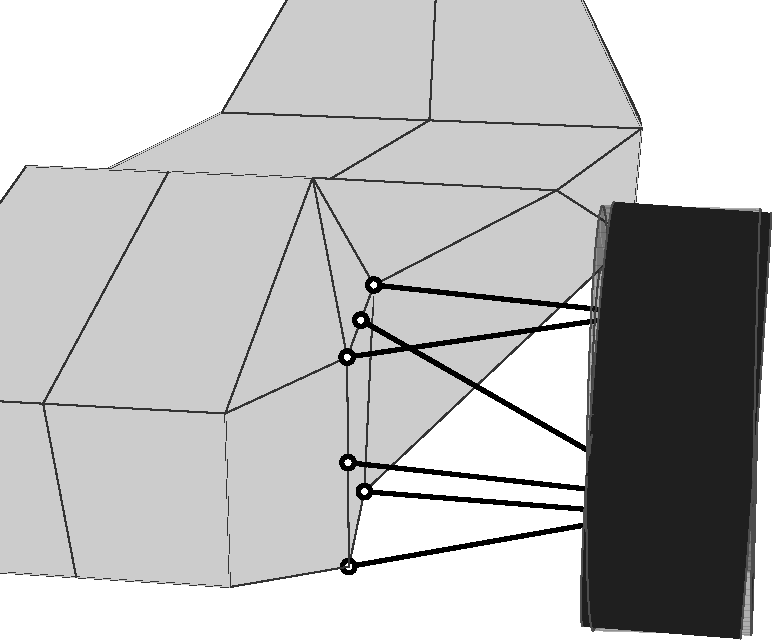
\includegraphics[scale = .6]{Images/camber_showing}
	\caption{Real scale representation of the wheel in two configurations: $q_{hk}=0$ (shaded surface) and $q_{hk}=-\pi/20$ (solid surface).}
	\label{fig:camber_showing}
\end{figure}
\subsection{External Wrenches}
\label{sec:extwren}
The external wrenches acting on each body, from wheels to chassis, are expressed in body-fixed components. Only gravity, aerodynamic forces, and road-tyre interactions are considered. Following~\cite{Guiggiani:book:2023}, the aerodynamic wrench in frame $\{B\}$ is $W_a=-\frac{1}{2}\rho S v_{gb,1}^2 [C_x, 0, C_z, 0, -h_0 C_x - a_f C_{zf} + a_r C_{zr}, 0]^T$, where $\rho$ is air density, $S$ is the frontal area, $v_{gb,1}$ the forward velocity (component of \emph{distal rigid-body twist} $V_{gb}$, see~\cite[p.~4]{Domenighini:Designs:2023}), and $C_x, C_z$ are drag/lift coefficients. $C_z$ is split into $C_{zf}=k_a C_z$ and $C_{zr}=(1-k_a)C_z$ by the aerodynamic balance coefficient $k_a$.

The total external wrench on a wheel is $W_{we}=\Ad_{g_{hn}}^*W_t+W_{w_h}$,
%\begin{equation}\label{eqn:Wwe}
%W_{we}=\Ad_{g_{hn}}^*W_t+W_{w_h},
%\end{equation}
where $W_t=[F_x, F_y, F_z, 0, 0, 0]^T$ is the ground wrench transferred from $\sref{N}$ to $\sref{H}$ by the \emph{starred} Adjoint operator, and $W_{w_h}=[F_{w_h}^T R_{hg}^T, 0, 0, 0]^T$ is the weight contribution with $F_{w_h}=[0, 0, -m_h g]^T$ in frame $\{G\}$, where $m_h$ is the wheel mass.

Knuckles experience no external forces, therefore:
\begin{equation}\label{eqn:Whe}
	W_{he}=[0,0,0,0,0,0]^T\quad\textrm{and}\quad W_{ke}=[0,0,0,0,0,0]^T.
\end{equation}
The chassis's external wrench is $W_{be}=W_a+W_{w_b}$, %\begin{equation}\label{eqn:Wbe}
%	W_{be}=W_a+W_{w_b},
%\end{equation}
where $W_a$ and $W_{w_b}$ are aerodynamic and weight contributions, respectively. For $W_{w_b}=[F_{w_b}^T R_{bg}^T, 0, 0, 0]^T$, the weight force is $F_{w_b}=[0, 0, -m_b g]^T$ in frame $\{G\}$, with $m_b$ as the chassis mass.
%The purpose of this section is to describe the external wrenches acting on each body, from the wheels to the chassis, each expressed in body-fixed components.
%Besides gravity, aerodynamic forces and the interactions between road and tyres are the only external forces considered.
%Adopting the notation in~\cite{Guiggiani:book:2023}, the aerodynamic contribution to the wrenches in frame $\{B\}$ is $W_a=-\frac{1}{2}\rho Sv_{gb,1}^2[C_x,0,C_z,0,-h_0C_x-a_fC_{zf}+a_rC_{zr},0]^T$, where $\rho$ is the air density, $S$ the frontal area of the vehicle, $v_{gb,1}$ the forward velocity, $h_0$ the nominal height of the CoM from ground and $a_f,a_r$ the distances of the CoM from the front and rear axle, respectively. The drag and lift coefficient $C_x$ and $C_z$ are dimensionless parameters that depend on the shape of the vehicle's body. $C_z$ can be further partitioned into $C_{zf}=k_a C_z$ and $C_{zr}=(1-k_a) C_z$ according to the \emph{aerodynamic balance coefficient} $k_a$, which is a parameter of the vehicle set-up.
%
%The total external wrench acting on a (general) wheel is:
%\begin{equation}\label{eqn:Wwe}
%	W_{we}=\Ad_{g_{hn}}^*W_t+W_{w_h},
%\end{equation}
%where $W_t=[F_x,F_y,F_z,0,0,0]^T$ are the ground forces computed in $\sref{N}$ and properly transferred to $\sref{H}$ components by the \emph{starred} Adjoint operator, while $W_{w_h} = [ F_{w_h}^T R^T_{hg}, 0,0,0 ]^T$, with $F_{w_h}=[0,0,-m_h g]^T$ in frame $\{G\}$, represents the weight contribution and $m_{h}$ is the wheel mass.
%
%Under our hypotheses, the knuckles are not subjected to external forces, thus \begin{equation}\label{eqn:Whe}
%	W_{he}=[0,0,0,0,0,0]^T\quad\textrm{and}\quad W_{ke}=[0,0,0,0,0,0]^T.
%\end{equation}
%
%The resultant external wrench acting on the chassis is therefore:
%\begin{equation}\label{eqn:Wbe}
%	W_{be}=W_a+W_{w_b},
%\end{equation}
%where $W_a$ and $W_{w_b}$ are, respectively, the contributions of aerodynamic and chassis weight forces, whose general expression is of the form $W_{w_b} = [ F_{w_b}^T R^T_{bg}, 0,0,0 ]^T$. Explicitly we have $F_{w_b}=[0,0,-m_b g]^T$ in frame $\{G\}$, where $m_b$ is the mass of the chassis.

\subsection{Recursive computation of the dynamics equations with ABA}
\label{sec:aba}
Thanks to the ABA algorithm, assuming known joint positions and velocities and joint forces and torques, it is possible to compute recursively and efficiently the accelerations of the joint variables. Following~\cite{Domenighini:Designs:2023}, twists are streamlined as follows: $V_{gb}^b = V_{gb} = V_b$, $V_{bh}^h=V_{bh}$, $V_{hw}^h=V_{hw}$. For the second model (DCC) the last expression is replaced with $V_{kw}^k=V_{kw}$ and $V_{hk}^k=V_{hk}$ is added. Given that the first model (without camber control) is a particular case of the DCC one, to avoid duplications only the algorithm for DCC is reported here.

The traditional ABA requires knowledge of the active forces and torques, denoted as $\tau_{ij}$, exerted by the parent body ($i$) on the child body ($j$). Its purpose is to solve the \emph{Forward Dynamics} problem of an articulated systems of rigid bodies. In our floating-base system, given the twist $V_b$ of the parent body $\{B\}$, the values and time derivatives of all joint variables ($q$ and $\dot{q}$), and the torque vector ($\tau$), the objective is to compute the joint accelerations ($\dot{V}_{b}$ and $\ddot{q}$).
%The fundamental concept is that of the inertia of an articulated body. This is represented by that of the root rigid body (original parent) plus the portion of the sub-trees, composed by the children bodies, whose inertia that can be structurally transferred backwards through the joints.
%This depends on the architecture, the pose and the joints' types.
The overall computation is performed in three sweeps defined recursively. One of the greatest computational benefits when it is employed to assemble symbolic dynamic equations, as in our case, is that \emph{no matrix inversion is required}, thus contributing to streamline the algebraic expressions.

The first step of the algorithm, as described in \textbf{Step 1}, performs the forward propagation of rigid-body velocities: from the root to the leaves of the tree.
%Twists are calculated as the sum of parent twist and the relative twist which is expressed consistently with the joint type. The interesting Jacobians are listed here: $J_{hk}=[0,0,0,1,0,0]^T$ and $J_{kw}=[0,0,0,0,1,0]^T$, and represent two revolute joints with axes $x$ and $y$ respectively.
In Algorithm~\ref{alg:step1} the terms ``Knuckle 1'' and ``Knuckle 2'' are used to identify the two halves of the knuckle, where, using kinematic trees terminology, the first is the parent of the second.
The Adjoint operator is defined as follows:
\begin{equation}\label{eq:Adjoint} \Ad_{g}=\left[\begin{array}{cc}R&\hat{d}R\\0&R\end{array}\right].
\end{equation}
In the case $g_{bh}\in SE(3)$ is considered, $R_{bh}\in SO(3)$ and $d_{bh}\in \bbR^3$ are functions of $(z,\delta)$. In the case of $g_{hk}$, the expressions are simply $d_{hk}=[0,0,0]^T$ and $R = \rotX(q_{hk})$, the latter being an elementary rotation about the common $x$-axis of the angle $q_{hk}$.

\begin{algorithm}[h]
	\floatname{algorithm}{Step}
	\caption{Forward Propagation of Velocity}\label{alg:step1}
	\begin{algorithmic}[1]
		\vspace{1mm}
		\For{$h=h_1,h_2,h_3,h_4$}
		\vspace{1mm}
		\State{$V_{bh}=J_{bh,z}\dot{z}+J_{bh,\delta}\dot{\delta}$}
		\vspace{1mm}
		\State{$V_h=\Ad_{g_{bh}}^{-1}V_b+V_{bh}$}\Comment{Knuckle 1 Rigid-Body Velocity}
		\vspace{1mm}
		\State{$V_{hk} = J_{hk}\dot{q}_{hk}$}
		\vspace{1mm}
		\State{$V_k=\Ad_{g_{hk}}^{-1}V_h+V_{hk}$}\Comment{Knuckle 2 Rigid-Body Velocity}
		\vspace{1mm}
		\State{$V_{kw}=J_{kw}\omega$}
		\vspace{1mm}
		\State{$V_w=V_k+V_{kw}$}\Comment{Rim Rigid-Body Velocity}
		\vspace{1mm}
		\EndFor
		\vspace{1mm}
	\end{algorithmic}
\end{algorithm}

The second step of the algorithm, as detailed in \textbf{Step 2}, performs the backward propagation of inertia and bias terms.
\begin{algorithm}[h]
	\floatname{algorithm}{Step}
	\caption{Backward Propagation of Articulated Inertia and Bias}\label{alg:step2}
	\begin{algorithmic}[1]
		\vspace{1mm}
		\For{$h=h_1,h_2,h_3,h_4$}
		\vspace{1mm}
		\State{$\hat{M}_w=M_w$}\Comment{Rim Articulated Inertia}
		\vspace{1mm}
		\State{$\hat{B}_w=-W_{we}+\ad_{V_w}^*M_wV_w$}\Comment{Rim Articulated Bias}
		\vspace{1mm}
		\State{$\bar{M}_w=\hat{M}_w-\dfrac{\hat{M}_wJ_{hw}J_{hw}^T\hat{M}_w}{J_{hw}^T\hat{M}_wJ_{hw}}$}
		\vspace{1mm}
		\State{$\bar{B}_w=\hat{B}_w-\dfrac{\hat{M}_wJ_{hw}J_{hw}^T\hat{B}_w}{J_{hw}^T\hat{M}_wJ_{hw}}-\bar{M}_w\ad_{V_{hw}}V_w$}
		\vspace{1mm}
		\State{$\hat{M}_k= \bar{M}_w$
		}\Comment{Knuckle 2 Articulated Inertia}
		\vspace{1mm}
		\State{$\hat{B}_k= \bar{B}_w$
		}\Comment{Knuckle 2 Articulated Bias}
		\vspace{1mm}
		\State{$\hat{M}_h= \Ad_{g_{hk}}^*\hat{M}_k\Ad_{g_{hk}}^{-1}$
		}\Comment{Knuckle 1 Articulated Inertia}
		\vspace{1mm}
		\State{$\hat{B}_h= \Ad_{g_{hk}}^*\bigl(\hat{M}_k(J_{hk}\ddot{q}_{hk}-\ad_{V_{hk}}\Ad_{g_{kh}}V_k)+\hat{B}_k\bigr)$
		}\Comment{Knuckle 1 Articulated Bias}
		\vspace{1mm}
		\State{$\bar{M}_h=\hat{M}_h-\dfrac{\hat{M}_hJ_{bh,z}J_{bh,z}^T\hat{M}_h}{J_{bh,z}^T\hat{M}_hJ_{bh,z}}$}
		\vspace{1mm}
		\State{$\bar{B}_h=\hat{B}_h-\dfrac{\hat{M}_hJ_{bh,z}(J_{bh,z}^T\hat{B}_h-\tau)}{J_{bh,z}^T\hat{M}_hJ_{bh,z}}-\bar{M}_h(\ad_{V_{bh}}V_h-\dot{J}_{bh,z}\dot{z}-\dot{J}_{bh,\delta}\dot{\delta}-J_{bh,\delta}\ddot{\delta})$}
		\vspace{1mm}
		\EndFor
		\vspace{1mm}
		\State{$\hat{M}_b=M_b+\displaystyle\sum_h\Ad_{g_{bh}}^*\bar{M}_h\Ad_{g_{bh}}^{-1}$}\Comment{Chassis Articulated Inertia}
		\vspace{1mm}
		\State{$\hat{B}_b=-W_{be}+\ad_{V_b}^*M_bV_b+\displaystyle\sum_h\Ad_{g_{bh}}^*\bar{B}_h$}\Comment{Chassis Articulated Bias}
		\vspace{1mm}
	\end{algorithmic}
\end{algorithm}

%Both inertia and bias are expressed in the body-fixed components.
In the case the DCC architecture is considered, the camber angle acceleration $\ddot{q}_{hk}$ is known, since $q_{hk(t)}$ is the assumed input, while the torque $\tau_{hk}$ has to be computed together with the rest of unknown accelerations, which are the outcome of the third sweep. This leads to a \emph{Hybrid Dynamics} problem that requires to carefully revisit the ABA's second and third steps.
The approach used is inspired by~\cite[Section~2.3]{Kim:notes:2012} where the the notation and conventions here employed were adapted according to~\cite{Domenighini:Designs:2023}.
%Specifically, apart from the labels assigned to the quantities, the primary difference between the two methods is the ordering of the twist vector. In this work, the twist vector is defined as $V = [v,\omega]^T$, whereas in the other method, it is defined as $V=[\omega,v]^T$. This difference might seem minor but leads to significant changes in the definitions of Adjoint operators, inertia matrices, bias and wrench vectors.

%For a generic articulated body the Newton-Euler equations can be expressed in the form:
%\begin{equation}\label{eqn:NE}
%	W=\hat{M}\dot{V}+\hat{B}.
%\end{equation}
%For a leaf node of the kinematic tree, having no children, the articulated inertia $\hat{M}$ is simply the generalized inertia $M$ of the body itself. Consistently, the bias $\hat{B}=B$, where:
%\begin{equation}
%	B=-W_e+\ad_V^*MV,
%\end{equation}
%and where $W_e$ is the resultant external wrench applied to the body and $\ad_V^*MV$ accounts for generalized gyroscopic and centrifugal forces, which are bi-linear in $V$. According to~\cite[Section~4.3.3]{Murray:book:1994} $\ad^*=-\ad^T$ has been defined. (If $v$ and $\omega$ are the translational and rotational component of $V$, then $\ad^*_V=\left[\begin{smallmatrix}\hat{\omega}&0\\\hat{v}&\hat{\omega}\end{smallmatrix}\right]$).

Starting from the leaf nodes, which in our case are represented by the wheels ($\sref{W}$), after providing information such as external wrenches, twists, joint geometry, body masses, joint forces / torques for traditional connections, and time evolution of variables defining kinematically imposed joints, the backward propagation of inertia and bias can be performed.

Finally the last step, denoted as \textbf{Step 3}, starting from the root node, computes joint variable accelerations and consequently body twists derivatives. For the kinematically controlled camber joints, the torques $\tau_{hk}$ needed to maintain the desired state of motion (DCC architecture) are computed as a by-product of the local inverse dynamics. This information is crucial to prevent actuators from  saturating or operating outside their bandwidth in the planned trajectories.

The root twist acceleration is determined by solving equation $W=\hat{M}\dot{V}+\hat{B}$, considering that the chassis is free-floating. The other unknown quantities, such as variable accelerations and torques, are computed projecting the Newton-Euler equations of each body along the respective Jacobian and then solving for the variable. See also~\cite{Domenighini:Designs:2023} for more details in the derivation of the equations.

\begin{algorithm}[h]
	\floatname{algorithm}{Step}
	\caption{Forward Propagation of Acceleration}\label{alg:step3}
	\begin{algorithmic}[1]
		\State{$\dot{V}_b=-\hat{M}_b^{-1}\hat{B}_b$}\Comment{Chassis Rigid-Body Acceleration}
		\vspace{1mm}
		\For{$h=h_1,h_2,h_3,h_4$}
		\vspace{1mm}
		\State{$\ddot{z}=-\dfrac{J_{bh,z}^T\bigl(\hat{B}_h+\hat{M}_h(\Ad_{g_{bh}}^{-1}\dot{V}_b-\ad_{V_{bh}}V_h+\dot{J}_{bh,z}\dot{z}+\dot{J}_{bh,\delta}\dot{\delta}+J_{bh,\delta}\ddot{\delta})\bigr)-\tau}{J_{bh,z}^T\hat{M}_hJ_{bh,z}}$}
		\vspace{1mm}
		\State{$\dot{V}_{bh}=\dot{J}_{bh,z}\dot{z}+\dot{J}_{bh,\delta}\dot{\delta}+J_{bh,z}\ddot{z}+J_{bh,\delta}\ddot{\delta}$}
		\vspace{1mm}
		\State{$\dot{V}_h=\Ad_{g_{bh}}^{-1}\dot{V}_b-\ad_{V_{bh}}V_h+\dot{V}_{bh}$}\Comment{Knuckle 1 Rigid-Body Acceleration}
		\vspace{1mm}
		\State{$\tau_{hk} = J_{hk}^T\bigl(\hat{B}_k+\hat{M}_k(\Ad_{g_{kh}}\dot{V}_h-\ad_{V_{hk}}V_k + J_{hk}\ddot{q}_{hk})\bigr)$}
		\vspace{1mm}
		\State{$\dot{V}_{bh} = J_{hk}\ddot{q}_{hk}$}
		\vspace{1mm}
		\State{$\dot{V}_k=\Ad_{g_{hk}}^{-1}\dot{V}_h-\ad_{V_{hk}}V_k+\dot{V}_{bh}$}\Comment{Knuckle 2 Rigid-Body Acceleration}
		\State{$\dot{\omega}=-\dfrac{J_{kw}^T\bigl(\hat{B}_w+\hat{M}_w(\dot{V}_k-\ad_{V_{kw}}V_w)\bigr)}{J_{kw}^T\hat{M}_wJ_{kw}}$}
		\vspace{1mm}
		\EndFor
		\vspace{1mm}
	\end{algorithmic}
\end{algorithm}

\subsection{Dynamic Model}
The dynamics equations, assembled via the procedure described  in Sec.~\ref{sec:aba}, are implemented in the software code by using a state-space representation $\dot{x}=f(x,u)$.
%\begin{equation}\label{eqn:f}
%	\dot{x}=f(x,u).
%\end{equation}
The state vector is $x = (q_{gb};V_{gb};z;\dot{z};\omega;q_{hk};\dot{q}_{hk})\in\bbR^{32}$, with components defined in previous sections. As already mentioned, in the model the camber joint is kinematically controlled as per the DCC architecture. Hence, the associated control vector is $u=(T_a;T_b;\delta;\ddot{q}_{hk})\in\bbR^{16}$, where each element is in $\bbR^{4}$ and collects the controls of the branch to each wheel. The torque is split into acceleration and braking components, allowing for minor modifications to model on-board motors coupled with traditional brakes and/or in-wheel motors as well. These components have their reaction torques in two different bodies in case of on-board motors and traditional brakes: the chassis and the knuckles, respectively. The $\delta$ vector collects the four translations of the steering rod attachment points, as described in Section~\ref{sec:suspanal}, while for the vector $\ddot{q}_{hk}$ no further explanation should be necessary. Clearly, this representation is valid for the model with active camber. The simpler model (no DCC) shares with the former the first 24 components of the state vector and the first 12 of the control vector.

The time derivative of the state vector has also been expressed previously except for the first element, $q_{gb}$. Its derivative is a function of the state and can be recovered using a standard procedure~\cite{Domenighini:Designs:2023} as follows:
\begin{equation}\label{eqn:dotqgb}
	\dot{q}_{gb}=J_{gb}^{-1}(q_{gb})V_{gb},
\end{equation}
where $J_{gb}(q_{gb})\in\bbR^{6\times6}$ is the Jacobian of the virtual joint connecting the ground to the chassis, and it is computed via the PoE parameterization of the transformation $g_{gb}$.
%, similarly to $J_{bh}$ in Eq.~\eqref{eqn:Jbh}. 
\section{Performance comparison} 
\label{sec:performance_comparison}

In this section we present some results obtained using the described robust planning frameworks. All planned trajectories refer to the sector of the Catalunya circuit shown in Figure~\ref{fig:track}. 
The entire circuit is parametrized by the curvilinear abscissa $\alpha \in [0,1]$, and the selected sector corresponds to the interval $\left[0.70, 0.77\right]$. Checkpoints are indicated by labels and are uniformly spaced by $\De\al=0.01$. This sector includes two distinct corners: a low-speed turn from $\al = 0.72$ to $\al = 0.73$, and a high-speed turn from $\al = 0.75$ to $\al = 0.76$, allowing for the evaluation of vehicle behavior across different dynamic scenarios.

We begin by presenting a selection of results obtained with the open-loop planning approach, which allows for a clearer illustration of the method and its underlying mechanisms. This approach is used as a reference to analyze the influence of key design parameters and of the different types of constraints on the resulting trajectories. A comparison is then carried out between the open-loop and closed-loop strategies. Finally, the planned trajectories are compared against those followed in simulations with noise realizations, providing empirical validation of the proposed framework.

% Contour plot dei LAP time in funzione dei due gamma, lo mettiamo o no? Eventialmente nel comparison open/closed

\begin{figure}
	\centering
	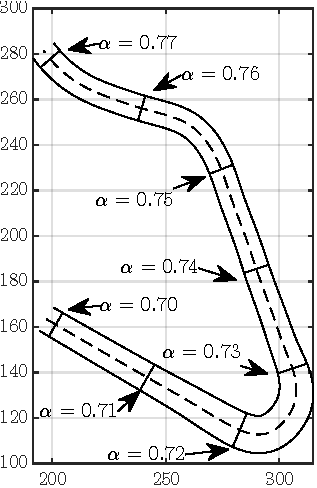
\includegraphics{Fig/track.pdf}
	\caption{Sector of the Catalunya circuit considered in the analysis, corresponding to the curvilinear abscissa interval $\left[0.70, 0.77\right]$. Checkpoints are indicated by labels and are uniformly spaced by $\De\al=0.01$. This sector includes two distinct corners: a low-speed turn from $\al = 0.72$ to $\al = 0.73$, and a high-speed turn from $\al = 0.75$ to $\al = 0.76$, allowing for the evaluation of vehicle behavior across different dynamic scenarios.}
	\label{fig:track}
\end{figure}

\subsection{Open-loop parameters sensitivity}
\label{sec:ol_param_sensitivity}
To gain deeper insight into how key parameters affect the planning outcome, we focus here on the open-loop formulation.
%In this section, we explore the open-loop approach to gain deeper insight into the influence of key parameters on the results.
At this stage, only the track limit constraint is robustified. 
%For this analysis, we consider optimizations in which only the track limit constraint is robustified. 
This choice is motivated by the fact that its effects are more visually evident than those of the friction limit constraint, thereby facilitating a more immediate understanding of their impact. 

The first parameter considered is the confidence level of constraint satisfaction. 
We recall that the factor $\ga^\textrm{TLC}$ acts as a tuning knob, multiplying the standard deviation of the constraint, $\sigma^\textrm{TLC}$, to determine the total back-off term $\be^\textrm{TLC}$. 
This parameter directly influences the probability of satisfying the track limit constraint: higher values of $\ga^\textrm{TLC}$ correspond to more conservative (i.e., robust) behavior. 
Specifically, $\ga^\textrm{TLC} = 0$ yields a satisfaction probability of 50\% and leads to the nominal solution with no back-off, while $\ga^\textrm{TLC} = 3$ corresponds to a confidence level of 99\%. 
For the purposes of this analysis, we examine the effect of varying $\ga^\textrm{TLC}$ across this range. 

%Setting $\ga^\textrm{TLC} = 0$ leads to the nominal solution. In this case, the back-off term $\be^\textrm{TLC}$ becomes zero, meaning that the constraint is not robustified and thus coincides with the original, non-robust formulation. 

Observing the left panel of Figure~\ref{fig:ol_sensitivities}, it is evident that the trajectories corresponding to configurations with lower values of $\ga^\textrm{TLC}$ tend to travel closer to the track boundaries. In contrast, the trajectory associated with $\ga^\textrm{TLC} = 3$---represented by the light green line---remains significantly farther from the edges.
This behavior is consistent with the increased conservativeness introduced by higher values of $\ga^\textrm{TLC}$, which amplify the back-off term $\be^\textrm{TLC}$ and thereby enforce a larger safety margin from the track limits.
Chasing a trajectory associated with a larger safety margin leads to higher sector times; spanning $\ga^\textrm{TLC}$ in the range $\left[0,3\right]$ results in sector times that vary from 12.135\,s to 13.162\,s.

\begin{figure}
	\centering
	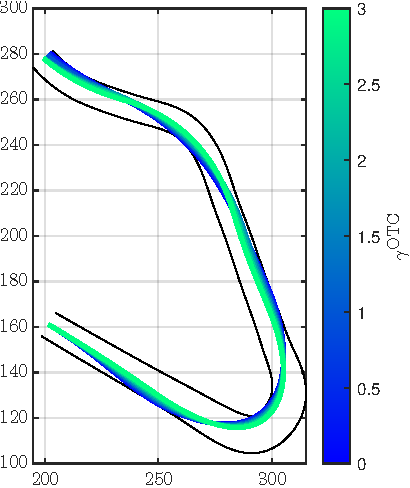
\includegraphics{Fig/gamma_sensitivity.pdf}
	\hfill
	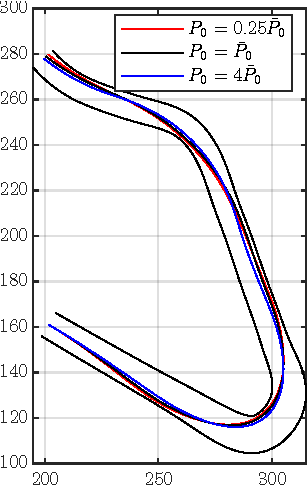
\includegraphics{Fig/Pzero_sensitivity.pdf}
	\caption{Effect of $\ga^\textrm{TLC}$ (left panel) and $P_0$ (right panel) on optimal trajectory. The parameter $\ga^\textrm{TLC}$ spans in the range $\left[0,3\right]$ corresponding to a probability to meet the track limit constraint ranging from 50\% to 99\%. In the right panel, in addition to the baseline value $\bar{\bP}_0$ (black line), two alternative values are considered: $\bP_0 = 4\bar{\bP}_0$ (blue line) and $\bP_0 = \frac{1}{4}\bar{\bP}_0$ (red line). These correspond, respectively, to doubling and halving the initial uncertainty associated with the state vector.}
	\label{fig:ol_sensitivities}
\end{figure}

The second parameter examined is the initial value of the covariance matrix, $\bP_0$. 
We recall that at each grid point a new prediction horizon is initialized, and the corresponding matrix $\bP$ at its starting point, i.e., $\bP^0_k$, is set to $\bP_0$. 
The diagonal elements of $\bP$ are the variances $\text{var}(x_i)$ of each state variables, while the off-diagonal elements encode their covariances $\text{cov}(x_i,x_j)$. Larger diagonal values indicate higher uncertainty in the corresponding states, and nonzero off-diagonal terms imply mutual dependence between them. For simplicity, a diagonal $\bP_0$ is used in this study, that is, for each prediction horizon we assign an initial standard deviation $\sigma_i = \sqrt{\text{var}(x_i)}$ to each state and assume all initial covariances to be zero. 

To provide a concrete interpretation, consider the first state variable $x_1$ with mean $\mu_1$ and standard deviation $\sigma_1$.
Under the Gaussian assumption, the true value of $x_1$ lies within the interval $\left[\mu_1 - \sigma_1,\ \mu_1 + \sigma_1\right]$ with approximately 68\% probability, and within the interval $\left[\mu_1 - 3\sigma_1,\ \mu_1 + 3\sigma_1\right]$ with approximately 99\% probability.

We assign a baseline initial covariance matrix $\bP_0 = \bar{\bP}_0$ by selecting standard deviations $\bar{\sigma}_i$ for each state variable. These standard deviations have been chosen based on the typical range of variation of each state.
Assuming the state vector is ordered as described in Section~\ref{sec:vehicle_model}, the values used are $\bar{\boldsymbol{\sigma}}~=~\left[0.1\,\textrm{m/s}, 0.01\,\textrm{m/s}, 0.01\,\textrm{rad/s}, 1\,\textrm{m}, 1\,\textrm{m}, 0.0175\,\textrm{rad}\right]^T$.
In addition to the baseline value $\bar{\bP}_0$, two alternative values are considered: $\bP_0 = 4\bar{\bP}_0$ and $\bP_0 = \frac{1}{4}\bar{\bP}_0$. These correspond, respectively, to doubling and halving the initial standard deviations $\sigma_i$ associated with the state vector. 

A comparison between the trajectories obtained using different values of $\bP_0$ is shown in the right panel of Figure~\ref{fig:ol_sensitivities}.
The black line corresponds to the baseline case with $\bP_0 = \bar{\bP}_0$, while the red and the blue lines represent the cases with $\bP_0 = \frac{1}{4}\bar{\bP}_0$ and $\bP_0 = 4\bar{\bP}_0$, respectively. As reasonably expected, using a larger initial covariance matrix results in a greater covariance matrix after $H$ steps, which in turn leads to a higher back-off term. This is reflected in the blue line, which travels closer to the centerline with respect to the other two lines.

\subsection{Robustified constraints comparison}
%It is of interest to analyze how a robustified constraint---or a combination of the two described in Sections~\ref{sec:FLC} and~\ref{sec:TLC}---influences the driving style. 
We now investigate how the inclusion of different kinds of robustified constraints---individually or in combination, as described in Sections~\ref{sec:FLC} and~\ref{sec:TLC}---influences the driving style. 
We compare the nominal feed-forward optimal trajectory, obtained without robustified constraints, with those resulting from a robustified track limit constraint (denoted as TLC), a robustified friction limit constraint (denoted as FLC), and a scenario where both constraints are robustified (denoted as TLC+FLC). All the optimization are obtained with the open-loop method described in Section~\ref{sec:open_loop_planning}, setting $H=4$, and $\ga^\textrm{TLC}=\ga^\textrm{FLC}=1.28$, corresponding to a 90\% probability of satisfying both constraints. 

\begin{figure}
	\centering
	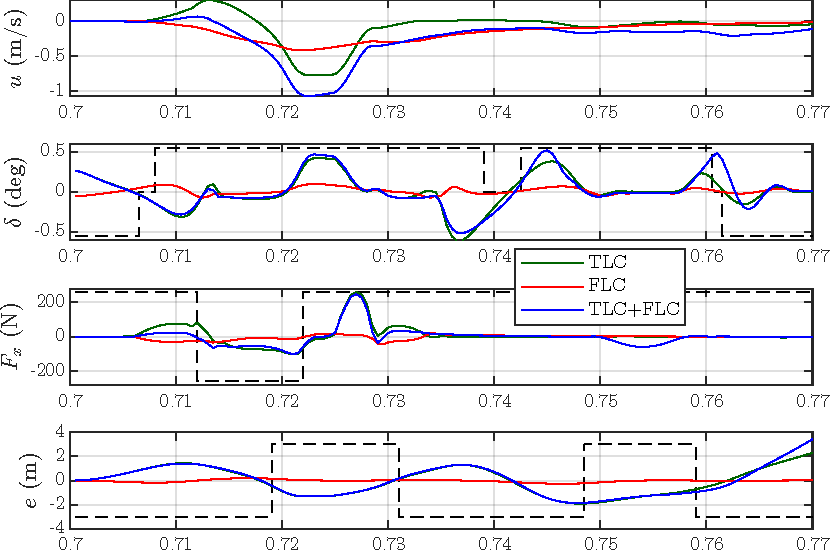
\includegraphics{Fig/ol_telemetries.pdf}
	\caption{Evolution of the longitudinal speed $\De u$, wheel steering angle $\De \de$, longitudinal force $\De F_x$, and lateral deviation $\De e$ are reported for three robustification scenarios: TLC (Track Limit Constraints), FLC (Friction Limit Constraint), and TLC+FLC (both constraints enforced concurrently). Each profile is shown relative to the baseline (nominal) trajectory to highlight the effect of each constraint-handling strategy. The dashed lines in the last three panels indicate the sign of the reference signal, allowing one to determine whether a positive variation with respect to the baseline corresponds to an increase or a decrease in the absolute value. This distinction is particularly important for quantities that depend on the direction of the turn, such as the wheel steering angle $\de$ and the lateral deviation $e$, while in the case of $F_x$, it indicates whether the vehicle is accelerating or braking.}
	\label{fig:ol_telemetries}
\end{figure}

%---Delta key signals

The comparison between the nominal case and the three robustified cases is illustrated in Figure~\ref{fig:ol_telemetries}, in terms of the deviation of selected signals from to their nominal counterparts.
The panels display variations on the longitudinal speed $\De u$ (first panel), wheel steering angle $\De \de$ (second panel), total longitudinal force $\De F_x$ (third panel), and lateral deviation of the center of mass (CoM) from the track centerline $\De e$ (fourth panel). 
Except for the $\De u$ panel, each plot includes dashed black lines that indicate the sign of the nominal signal. 
These indicators are shown at three distinct vertical levels---upper, central, and lower---corresponding respectively to positive, near-zero, and negative values of the nominal signal.

%--------1 Considerazioni generali sul settore

From the first panel, it can be observed that all robustified configurations, on average, show a lower longitudinal speed compared to the nominal trajectory, resulting in an increased sector time. Specifically, the configuration with the robustified TLC increases the sector time by 1.66\%, while that with the robustified FLC leads to a 0.79\% increase. When both TLC and FLC are robustified, the sector time increases by 2.57\%.
The two configurations incorporating the robustified TLC (blue and green lines) exhibit, as expected, a significantly altered CoM trajectory.
Ideed, the second and fourth panels clearly show that the TLC and TLC+FLC configurations tend to follow a path closer to the centerline. In particular, for most of the sector, the variation in lateral displacement $\De e$ and the lateral displacement $e$ itself exhibit opposite signs, indicating a corrective behavior of the steering angle $\de$ that pulls the vehicle toward the centerline.

%--------2 Sharp turn

This shift in trajectory and longitudinal speed becomes especially evident when approaching the sharp turn at $\al \in [0.707, 0.712]$. A noticeable increase in longitudinal speed is observed around $\alpha = 0.71$ for the TLC configuration  in the $\De u$ panel. This peak is followed by a sharp drop in speed, indicating intense braking.
The TLC+FLC configuration exhibits a qualitatively similar trend in $\Delta u$, although the peak is significantly lower and the subsequent speed reduction is clearly stronger. This behavior is consistent with the variation of the total longitudinal force $\Delta F_x$ shown in the third panel.
In particular, the TLC and TLC+FLC configurations exhibit a higher longitudinal force while approaching the sharp turn, in the curvilinear abscissa interval $\al\in\left[0.707, 0.712\right]$, resulting in a higher longitudinal speed.
Subsequently, these two configurations apply a lower longitudinal force during braking compared to the nominal case, indicating more intense braking. This behavior explains the sharp reduction in longitudinal speed observed thereafter.

%--------3 High speed turn

Later in the sector, a further deviation in driving style appears during the high-speed turn, specifically around $\alpha \in [0.75, 0.76]$.
As shown in the $\Delta F_x$ panel, the combined configuration TLC+FLC needs to reduce the longitudinal force within this section to meet both the constraints. 
This adaptation is necessary because the TLC forces the vehicle to follow a wider trajectory, which entails greater lateral acceleration and, consequently, higher lateral force demand. To satisfy the FLC under the resulting increase in tire utilization, the available accelerating force must be reduced.
Based on the nominal force sign indicator, this reduction is achieved by partially lifting the throttle.

%---Axle saturation
After analyzing the variations of these four key signals with respect to the nominal solution, we now turn our attention to the evaluation of axle saturation, which provides insight into how close each configuration operates to the tire grip limits. 
In accordance with the FLC formulation introduced in~\ref{eq:adherence_constraint}, we define the \emph{axle saturation ratio} $S_j$ as
\begin{equation}
	S_j = \frac{ \left( \frac{X_j(\bx,\bu)}{\mu_{x,j}} \right)^2+ \left( \frac{Y_j(\bx,\bu)}{\mu_{y,j}}\right)^2}{Z_j^2(\bx,\bu)}.
\end{equation}
This quantity indicates how close each configuration operates to the friction limit; $S_j = 1$ when the point $\left(X_j, Y_j\right)$ lies exactly on the friction ellipse, i.e., under full saturation.
Figure~\ref{fig:ol_saturation} shows the values of $S_j$ for the front axle ($j=1$, first panel) and the rear axle ($j=2$, rear panel) for the previously introduced configurations: the nominal case (black dashed line) and the three robustified cases (color-coded as before).

\begin{figure}
	\centering
	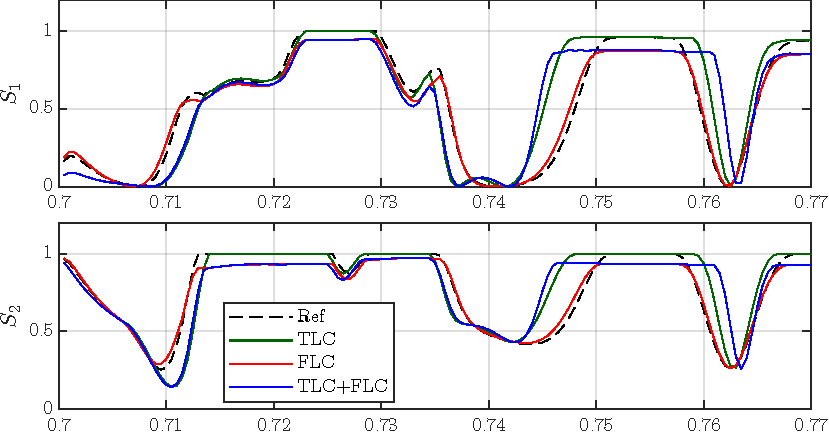
\includegraphics{Fig/ol_saturation.pdf}
	\caption{Tire usage for front axle (first panel) and rear axle (second panel) over curvilinear abscissa $\al$. The plotted lines represent the quantity $\left[ \left( \frac{X_j(\bx,\bu)}{\mu_{x,j}} \right)^2+ \left( \frac{Y_j(\bx,\bu)}{\mu_{y,j}}\right)^2\right]\frac{1}{Z_j^2(\bx,\bu)}$, where $j=1$ denotes the front axle and $j=2$ the rear axle. The dashed black line corresponds to the reference (nominal) configuration, while the green, red, and blue lines represent the robust configurations TLC, FLC, and TLC+FLC, respectively.}
	\label{fig:ol_saturation}
\end{figure}

First, we observe that the FLC and TLC+FLC configurations (red and blue lines) never reach full saturation, i.e., $S_j=1$, due to the presence of the back-off term, which enforces a safety margin from the friction limit. 
Second, we point out how the different trajectories followed by the TLC and TLC+FLC configurations (green and blue lines), compared to the nominal and FLC cases, entail distinct ground force demands, which are clearly visible here in terms of the $S_j$ ratio.
This behavior emerges around the sharp turn and becomes even more evident in the high-speed turn. 
Specifically, in the interval $\alpha \in [0.745, 0.762]$, the TLC and TLC+FLC configurations begin to experience high axle loads approximately 12\,m before the nominal trajectory and sustain them for an additional 4.6\,m (TLC, green line) and 9.2\,m (TLC+FLC, blue line) beyond the nominal reference. 


%As already observed, the configurations with the robustified track limit constraint (green and blue lines) follow significantly different paths compared to the nominal solution. This deviation results in distinct ground force demands, clearly visible in the saturation index.
%From this plot, it can be observed that the configurations with the robustified track limit constraint (green and blue lines) follow significantly different trajectories compared to the nominal solution, resulting in distinct ground force demands. This behavior is noticeable in turn 1 and even more clearly in turn 2. Specifically, these two configurations begin to experience high axle loads approximately 12\,m before the nominal trajectory and sustain them for an additional 4.6\,m (TLC, green line) and 9.2\,m (TLC+FLC, blue line) beyond the nominal reference. 

\subsection{Comparison between open-loop and closed-loop approaches}

\subsection{Simulations with noise realization}
This analysis aims to provide empirical validation of the robust trajectories obtained using the methods proposed in this work. For conciseness, the comparison is limited to a nominal trajectory and a trajectory computed using the closed-loop method with only the track limit constraint robustified.
An LQR controller, designed according to the procedure outlined in Section~\ref{sec:LQR}, is implemented to stabilize the nominal trajectory. In contrast, the robust trajectory is tracked using the controller directly obtained from the optimization process. 

\begin{figure}
	\centering
	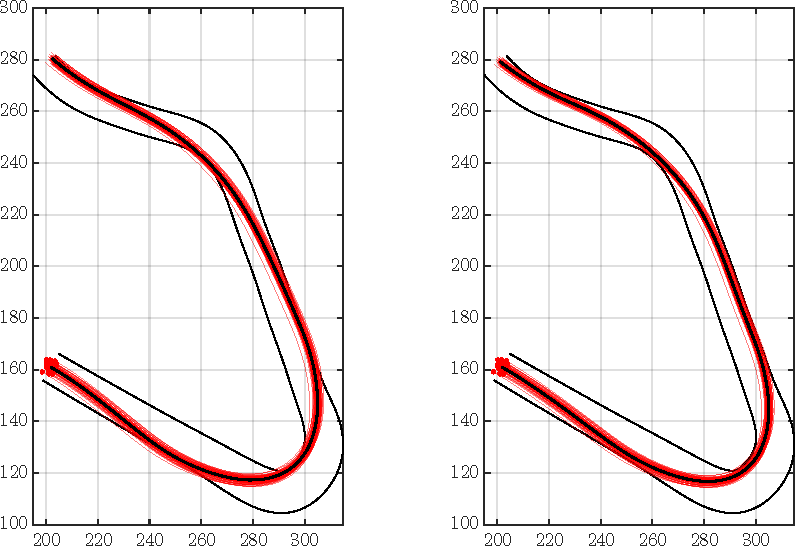
\includegraphics{Fig/olcl_traj_strings.pdf}
	\caption{Simulations with random initial conditions and Gaussian noise realizations. In the left panel, the reference trajectory is the non-robust one, tracked using an LQR controller designed around it. In the right panel, the reference is a robust trajectory obtained using the closed-loop optimization method, and it is tracked using the corresponding optimized controller produced by the same method.}
	\label{fig:traj_strings}
\end{figure}
\section{Conclusions} 
\label{sec:conclusions}

\section*{Acknowledgement(s)}

The authors would like to thank Dr. Lorenzo Bartali for his significant contributions to the initial version of the optimization framework developed and utilized in this paper.


\section*{Disclosure statement}

No potential conflict of interest was reported by the author(s).

\section*{Funding}

This work is supported by project PRIN 2022 PNRR ``Global Stability of road vehicle motion - STAVE'' CUP I53D23005670001.



%\section*{Notes on contributor(s)}
%
%An unnumbered section, e.g.\ \verb"\section*{Notes on contributors}", may be included \emph{in the non-anonymous version} if required. A photograph may be added if requested.
%
%
%\section*{Nomenclature/Notation}
%
%An unnumbered section, e.g.\ \verb"\section*{Nomenclature}" (or \verb"\section*{Notation}"), may be included if required, before any Notes or References.
%
%
%\section*{Notes}
%
%An unnumbered `Notes' section may be included before the References (if using the \verb"endnotes" package, use the command \verb"\theendnotes" where the notes are to appear, instead of creating a \verb"\section*").


\bibliographystyle{tfnlm}
\bibliography{biblio}


%\bigskip
%
%
%\section{Appendices}
%
%\appendix
%\chapter{First Algorithm}
%\label{app:alg}
%\begin{algorithm}[h]
%	\floatname{algorithm}{Step}
%	\caption{Forward Propagation of Velocity}\label{alg:step1_app}
%	\begin{algorithmic}[1]
	%		\vspace{1mm}
	%		\For{$h=h_1,h_2,h_3,h_4$}
	%		\vspace{1mm}
	%		\State{$V_{bh}=J_{bh,z}\dot{z}+J_{bh,\delta}\dot{\delta}$}
	%		\vspace{1mm}
	%		\State{$V_h=\Ad_{g_{bh}}^{-1}V_b+V_{bh}$}\Comment{Knuckle Rigid-Body Velocity}
	%		\vspace{1mm}
	%		\State{$V_{hw}=J_{hw}\omega$}
	%		\vspace{1mm}
	%		\State{$V_w=V_h+V_{hw}$}\Comment{Rim Rigid-Body Velocity}
	%		\vspace{1mm}
	%		\EndFor
	%		\vspace{1mm}
	%	\end{algorithmic}
%\end{algorithm}
%
%\begin{algorithm}[h]
%	\floatname{algorithm}{Step}
%	\caption{Backward Propagation of Articulated Inertia and Bias}\label{alg:step2_app}
%	\begin{algorithmic}[1]
	%		\vspace{1mm}
	%		\For{$h=h_1,h_2,h_3,h_4$}
	%		\vspace{1mm}
	%		\State{$\hat{M}_w=M_w$}\Comment{Rim Articulated Inertia}
	%		\vspace{1mm}
	%		\State{$\hat{B}_w=-W_{we}+\ad_{V_w}^*M_wV_w$}\Comment{Rim Articulated Bias}
	%		\vspace{1mm}
	%		\State{$\bar{M}_w=\hat{M}_w-\dfrac{\hat{M}_wJ_{hw}J_{hw}^T\hat{M}_w}{J_{hw}^T\hat{M}_wJ_{hw}}$}
	%		\vspace{1mm}
	%		\State{$\bar{B}_w=\hat{B}_w-\dfrac{\hat{M}_wJ_{hw}J_{hw}^T\hat{B}_w}{J_{hw}^T\hat{M}_wJ_{hw}}-\bar{M}_w\ad_{V_{hw}}V_w$}
	%		\vspace{1mm}
	%		\State{$\hat{M}_h= \bar{M}_w$
		%		%\State{$\hat{M}_h= M_h +\bar{M}_w$
			%		}\Comment{Knuckle Articulated Inertia}
		%		\vspace{1mm}
		%		\State{$\hat{B}_h=-W_{he}+\bar{B}_w$
			%			%\State{$\hat{B}_h=-W_{he}+\ad^{*}_{V_h} M_hV_h+\bar{B}_w$
				%			}\Comment{Knuckle Articulated Bias}
			%			\vspace{1mm}
			%			\State{$\bar{M}_h=\hat{M}_h-\dfrac{\hat{M}_hJ_{bh,z}J_{bh,z}^T\hat{M}_h}{J_{bh,z}^T\hat{M}_hJ_{bh,z}}$}
			%			\vspace{1mm}
			%			\State{$\bar{B}_h=\hat{B}_h-\dfrac{\hat{M}_hJ_{bh,z}(J_{bh,z}^T\hat{B}_h-\tau)}{J_{bh,z}^T\hat{M}_hJ_{bh,z}}-\bar{M}_h(\ad_{V_{bh}}V_h-\dot{J}_{bh,z}\dot{z}-\dot{J}_{bh,\delta}\dot{\delta}-J_{bh,\delta}\ddot{\delta})$}
			%			\vspace{1mm}
			%			\EndFor
			%			\vspace{1mm}
			%			\State{$\hat{M}_b=M_b+\displaystyle\sum_h\Ad_{g_{bh}}^*\bar{M}_h\Ad_{g_{bh}}^{-1}$}\Comment{Chassis Articulated Inertia}
			%			\vspace{1mm}
			%			\State{$\hat{B}_b=-W_{be}+\ad_{V_b}^*M_bV_b+\displaystyle\sum_h\Ad_{g_{bh}}^*\bar{B}_h$}\Comment{Chassis Articulated Bias}
			%			\vspace{1mm}
			%	\end{algorithmic}
		%\end{algorithm}
		%
		%\begin{algorithm}[h]
		%	\floatname{algorithm}{Step}
		%	\caption{Forward Propagation of Acceleration}\label{alg:step3_app}
		%	\begin{algorithmic}[1]
			%		\State{$\dot{V}_b=-\hat{M}_b^{-1}\hat{B}_b$}\Comment{Chassis Rigid-Body Acceleration}
			%		\vspace{1mm}
			%		\For{$h=h_1,h_2,h_3,h_4$}
			%		\vspace{1mm}
			%		\State{$\ddot{z}=-\dfrac{J_{bh,z}^T\bigl(\hat{B}_h+\hat{M}_h(\Ad_{g_{bh}}^{-1}\dot{V}_b-\ad_{V_{bh}}V_h+\dot{J}_{bh,z}\dot{z}+\dot{J}_{bh,\delta}\dot{\delta}+J_{bh,\delta}\ddot{\delta})\bigr)-\tau}{J_{bh,z}^T\hat{M}_hJ_{bh,z}}$}
			%		\vspace{1mm}
			%		\State{$\dot{V}_{bh}=\dot{J}_{bh,z}\dot{z}+\dot{J}_{bh,\delta}\dot{\delta}+J_{bh,z}\ddot{z}+J_{bh,\delta}\ddot{\delta}$}
			%		\vspace{1mm}
			%		\State{$\dot{V}_h=\Ad_{g_{bh}}^{-1}\dot{V}_b-\ad_{V_{bh}}V_h+\dot{V}_{bh}$}\Comment{Knuckle Rigid-Body Acceleration}
			%		\vspace{1mm}
			%		\State{$\dot{\omega}=-\dfrac{J_{hw}^T\bigl(\hat{B}_w+\hat{M}_w(\dot{V}_h-\ad_{V_{hw}}V_w)\bigr)}{J_{hw}^T\hat{M}_wJ_{hw}}$}
			%		\vspace{1mm}
			%		\EndFor
			%		\vspace{1mm}
			%	\end{algorithmic}
		%\end{algorithm}
		\section{Smoothing Function}\label{app:smoothing_functions}
		The optimizer, in order to find the solution, calculates several number of derivatives, hence, having differentiable function, possibly of class $C^\infty$, improves the quality of the solution and reduces the simulation time. 
		
		Here is proposed a smooth step function, used to perform comparison between decision variables, that exploits hyperbolic functions. 
		\begin{equation}\label{eq:ifelsesmooth}
			z = \frac{T}{2}\left[1 + \tanh(C\left(x-y\right))\right] + \frac{F}{2}\left[1 - \tanh(C\left(x-y\right))\right],
		\end{equation}
		where $T$ and $F$ represent the asymptotic values of the function when $x>y$ and $x<y$, respectively, while $C$ is a constant used to tune the hardness of the intervention. 
		Supposing to model an absolute value of $x$, setting $T=1$, $F=-1$, and $C=10$, reducing $z$ to depend only on $x$, the function can be expressed as follows:
		\begin{equation}
			\tilde{abs}(x) = z(x)\cdot x.
		\end{equation}
		
		\begin{figure}[h]
			\centering
			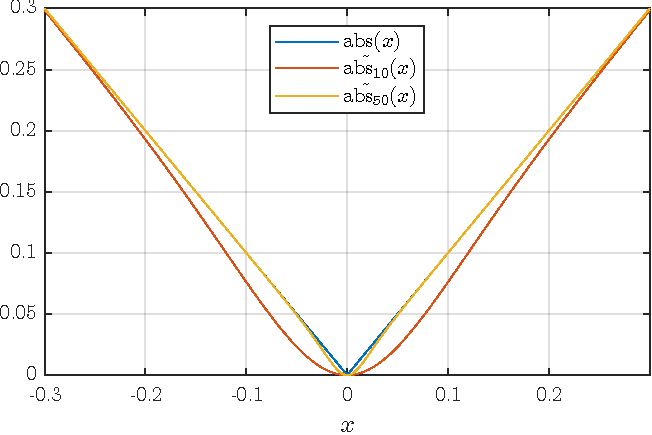
\includegraphics[scale = .8]{Images/Appendices/abs_smooth.pdf}
			\caption{Comparison between non derivable abs function (in blue) and two smooth abs functions (in red and yellow). The subscript on the smooth function indicates the value of the constant $C$, which tunes the hardness of the intervention. Increasing this value leads to a more accurate function, but results in higher derivatives as a drawback.}
			\label{fig:abs_smooth}
		\end{figure}

%\section{Troubleshooting}




%\section{Obtaining the template and class file}
%
%\subsection{Via the Taylor \& Francis website}
%
%...
%
%
%\subsection{Via e-mail}

\end{document}
